\chapter{Indledning}
I dette projekt er der arbejdet med design og udvikling af et blodtryksmålesystem. Ideen bag vores system blev udtænkt og udarbejdet med viden om en blodtryksmåler på en operationsstue på Herning Sygehus. Vores opstillede krav samt design til systemet, blev derfor lavet ud fra de oplysninger vi fik af en sygeplejerske\footnote{Anæstesisygeplejerske Charlotte Høj, Herning Sygehus} på Herning Sygehus. Der var et ønske om at lave et blodtryksmålesystem, som er så virkelighedsnært som muligt. Det design og den funktionalitet der blev efterstræbt i dette projekt, var at præsentere et blodtrykssignal, hvor det systoliske samt det diastoliske blodtryk kan bestemmes. Desuden få præsenteret et EKG-signal, hvorfra pulsen kan bestemmes, og præsentere iltmætningen i blodet for patienten. Vi ønsker at få vist grafer og værdier på en brugergrænseflade, som lever op til de standarder, der ses på operationsstuer i dag. \\
\\
Baggrunden for dette projekt er, at man i klinisk praksis har behov for kontinuert at observere patientens blodtryk. Det er i særdeleshed på intensiv afdelinger og operationsstuer, at man ønsker at lave direkte invasiv blodtryksmåling. Ved invasiv blodtryksmåling kan man monitorere patientens fysiske tilstand under eksempelvis en operation. Blodtrykket kan give en indikation om blødninger, smerter og hvor dybt patienten sover under narkosen. Denne overvågning giver det sundhedsfaglige personale en ekstra tryghed og sikkerhed om patientens tilstand under operation. \\
\\
Denne projektrapport vil give en kort beskrivelse af vores samlede system samt krav hertil. Der vil være en udspecificeret projektbeskrivelse, som vil give et indblik i vores vej frem til det endelige resultat. Den vil også beskrive de til- og fravalg vi har måttet tage, for at nå frem til det system, der kunne realiseres og præsenteres. Der har i den forbindelse været nogle ideer, som ikke har været realistiske og tidsmæssigt mulige at opfylde, og vil derfor være beskrevet i fremtidigt arbejde. Slutteligt vil der være en samlet konklusion på projektarbejdet.
\chapter{Projektformulering og afgrænsning}
I dette projekt udarbejdes et produkt, der kan måle blodtrykket for en patient og vise dette løbende på en graf. Desuden skal produktet kunne bestemme det diastoliske og systoliske tryk ud fra blodtrykskurven, ud fra disse trykværdier bestemmes middeltrykket. Ud fra systolisk og diastolisk tryk skal produktet kunne vise om en eller begge har overskredet en grænseværdi og signalere dette til det sundhedsfaglige personale. Produktet skal kunne filtrere det indhentede signal med et digitalt filter, sådan at signalet kan vises filtreret og ufiltreret.  \\\\
Dette betyder at produktet skal kunne:
\begin{itemize}
\item Indhente et blodtrykssignal igennem hardwaren, hvilken består af:
\begin{itemize}
\item Væskefyldt kateter
\item Transducer 
\item Forstærker
\item Lavpas filter
\item Spændingsforsyning
\item NI-DAQ
\end{itemize}
\item Vise blodtrykskurven kontinuert
\item Vise blodtrykskurven både filtreret og ufiltreret
\item Bestemme systolisk tryk
\item Bestemme diastolisk tryk
\item Bestemme middeltryk
\item Starte alarm, hvis systolisk/diastolisk tryk har overskredet en grænseværdi
\item Gemme blodtryksdata i en database
\end{itemize}
Løsningen til dette produkt har for vores vedkommende været et software og et hardware produkt, hvilke benyttes sammen til at indhente, behandle og vise blodtrykssignalet. Hardwaren bruges til at indhente og behandle blodtrykssignalet, sådan at dette signal kan sendes til softwaren. Softwaren skal kunne viderebehandle signalet, sådan at det indlæste signal kan præsenteres efter de opsatte krav. Softwaren skal have en brugergrænseflade, som bruges til at præsentere blodtrykssignalet for det sundhedsfaglige personale. \\
Ligeledes er det et ønske at produktet skal indhente EKG-signalet og iltsaturationen fra patienten. Disse data skal også kunne vises på en brugergrænseflade. Ud fra EKG-signalet bestemmes pulsen, altså hjertefrekvensen, for patienten, pulsen kan dog også bestemmes ved at finde antallet af systoler pr. minut, denne værdi præsenteres som talværdi på brugergrænsefladen. Ud fra iltsaturationen kan iltmætningen for blodet bestemmes, hvilken ligeledes præsenteres på brugergrænsefladen. 
\section{Oversigt over projektdeltagere og hovedansvarsområder}
I dette projekt er det valgt at dele projektets deltagere op i to grupper med hver deres hovedansvarsområder. Den ene gruppe har beskæftiget sig med hardware og den anden gruppe med software. Derudover blev der i starten af forløbet valgt en projektleder, hvis opgaver bestod i at lave dagsorden for hvert møde, sørge for at deadlines blev overholdt, træffe endelige beslutninger og have et overblik over projektet. En procesleder blev ligeledes valgt, hvis opgaver bestod i opgavestyring, godt arbejdsmiljø i gruppen og planlægning af projektforløbet. \\
Herunder ses de forskellige gruppemedlemmers hovedområde:\\\\
\begin{tabular}{| l | l |} \hline
\textbf{Hardware} & \textbf{Software}\\\hline
Brian Hansen & Ida Mark Skovbjerg \\\hline 
Mohamed Hussein Mohamed & Mette Østergård Knudsen \\\hline
Khaled Edwan & Line Skov Larsen  \\\hline 
\end{tabular}
\\\\
Gruppens medlemmer med fulde navn og initialer ses herunder:: \\\\
\begin{tabular}{| l | l |} \hline
\textbf{Fulde navn} & \textbf{Initialer}\\\hline
Ida Mark Skovbjerg & IMS \\\hline 
Line Skov Larsen & LL \\\hline
Mette Østergård Knudsen & MK  \\\hline 
Brian Hansen & BH \\\hline
Mohamed Hussein Mohamed & MM \\\hline 
Khaled Edwan & KE \\\hline
\end{tabular}
\chapter{Hjertet}
Hjertet er en muskel, der fungerer som en pumpe i kroppen. Hjertet pumper det iltede blod (arterielt blod) ud til resten af kroppen gennem arterie- og vene systemet. Når blodet passerer ud af hjertet igennem arterierne, sker der et tryk mod arterievæggene, dette tryk kaldes blodtrykket. \\\\
Hjertet opdeles i to adskilte hjertehalvdele, som fungerer som pumpe. Den venstre, som pumper blodet rundt i organismen og den højre, som pumper blodet gennem lungerne. De to hjertehalvdele er sammensat af atrier og ventrikler. Blodet fra organismen der føres tilbage til hjertet, er det venøse blod, som føres til højre atrium gennem øvre og nedre hulvene. Mellem højre atrium og højre ventrikel sidder trikuspidalklappen, som forhindrer blodet i at løbe tilbage til atriet under hjertets sammentrækning. Højre ventrikel udløber i lungepulsåren, som deles ud i hver lunge. Mellem ventriklen og lungepulsåren er pulmonalklappen, som forhindrer blodet i tilbageløb. I lungerne afgiver blodet CO$_{2}$ og optager ilt, denne diffusion af disse gasser sker i lungernes alveoler. Det nu iltrige blod returneres gennem lungevenerne til venstre atrium. Fra venstre atrium til venstre ventrikel sidder mitralklappen. Fra venstre ventrikel pumpes blodet ud i aorta gennem aortaklappen, herfra pumpes blodet rundt i resten af organismen. \cite{hjertedsd}
\begin{figure}[H]
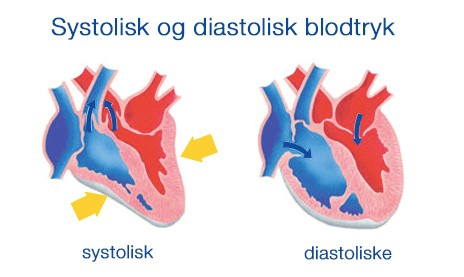
\includegraphics[width =0.5\textwidth , center]{billeder/sysdia}
\caption{\textbf{Hjertet ved systolisk og diastolisk blodtryk.\cite{hjertet}}}
\end{figure}
\newpage
\section{Blodtryk}
Blodtrykket ses når hjertets venstre hjerteventrikel trækker sig sammen, og der som resultat heraf, bliver presset blod ud i arterierne. Trykket vil altså være størst i arterierne, da arterierne er de blodåre som fører væk fra hjertet. Det laveste blodtryk vil være at se i venerne, da det er de blodårer, som fører blodet tilbage til hjertet. Blodtrykket vises som to værdier: systolen, som er hjertets sammentrækningsfase og diastolen som er hjertets afslapningsfase. \\\\
Systolen angives som den kraft, der skabes når der kommer pres på karvæggene i arterierne. Dette sker i hjertets sammentrækningsfase, hvor blodet pumpes ud i arterierne. Systolen i et normalt blodtryk i hvile vil ligge i intervallet 100-140 mmHg og ved forhøjet blodtryk er værdien for systolen over 140 mmHg.\\ Diastolen angiver hjertets hvilefase og ses mellem to sammentrækninger. I denne fase fyldes ventriklerne med blod. Den normale værdi for diastolen ligger i intervallet 60-90 mmHg. Hvis den overstiger 90 mmHg anses blodtrykket for at være forhøjet. Udover systolen og diastolen kan middeltrykket også angives. Dette udregnes ved $Middeltryk = \dfrac{2}{3}\cdot Diastole + \dfrac{1}{3}\cdot Systole$ \cite{blodtrykwiki}\\
Hypertension defineres som forhøjet systole, forhøjet diastole eller både forhøjet systole og diastole. Hypertension belaster hjertet, og kan medføre en øget risiko for udviklingen af apopleksi, arteriosklerose, hjerteinsufficiens og nyreskader. \cite{pulmonal}\\
Hvis værdien for systolen kommer under 100 mmHg og/eller diastolen kommer under 60 mmHg, vil der være tale om et for lavt blodtryk, hypotension. Lavt blodtryk behøver dog ikke at være alvorligt, men kan være helt normalt for f.eks. høje personer. Men i forbindelse med sygdom, traumer eller medicinoverdosering er hypotension en alvorlig tilstand. Hypotension ses bl.a. ved diabetes, traumer, hjertesvigt og Addisons sygdom. \cite{hypo}
\\\\
Anatomien bag blodtrykket og blodtryksændring, omfatter blodets kredsløb, hjertet og lymfesystemet. Blodkredsløbet er et langt netværk af arterier og vener, som har til opgave at føre iltet blod ud til hver celle i kroppen via kapillærerne, samt opfange affaldsprodukter fra celler og væv.\cite{pulmonal}  I lungekredsløbet udskilles CO$_2$ og blodet iltes. Det er hjertet der pumper blodet ud i dette netværk, så blodet hele tiden er i bevægelse. Arterierne transporterer blodet væk fra hjertet, og venernes opgave er at transportere blodet mod hjertet. 
\begin{figure}[H]
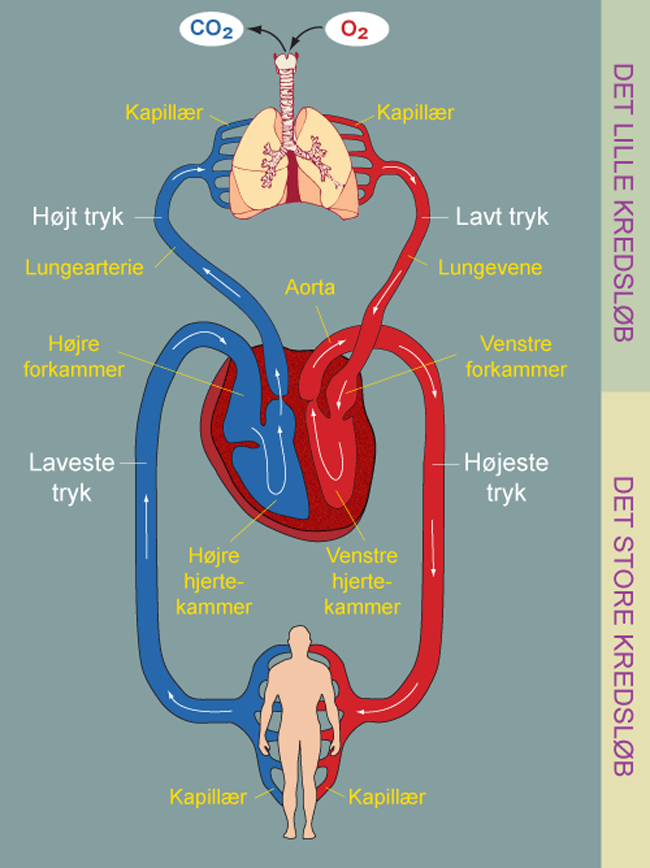
\includegraphics[width =0.5\textwidth , center]{billeder/hjertet}
\caption{\textbf{Det lille og det store kredsløb. Motoren der driver det hele er hjertet. \cite{hjertet}}}
\end{figure}
\section{Direkte invasiv måling af blodtryk}
Den mest almindelig metode til klinisk at måle blodtrykket, er ved at koble det vaskulære tryk til en extravaskulær sensor via et væskefyldt kateter. Klinisk er dette system påsat patientens a. Radialis via en arteriekanyle. Kateterslangen er forbundet til en trevejs stophane og videre til tryksensoren. Kateter-sensor systemet er fyldt med en saltvandsopløsning fra væskesøjlen.
\begin{figure}[H]
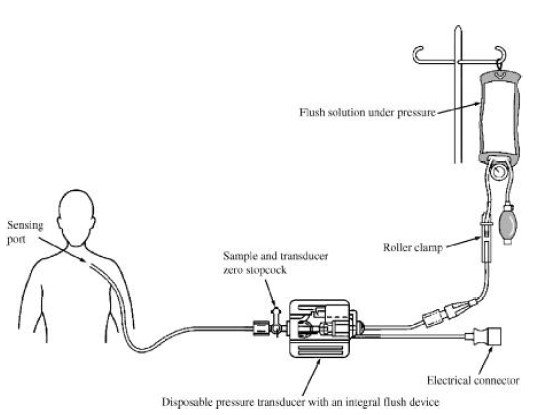
\includegraphics[width =0.7\textwidth , center]{billeder/kateter}
\caption{\textbf{Opstilling af direkte invasiv blodtryksmåling.}}
\end{figure}
Som det ses på figuren er sansningsporten indgangen til patients arterie. Kateteret er koblet til trevejs stophanen og videre til sensoren. Trevejs stophanen har tre mulige funktioner, 1: Der kan lukkes for blodtilførslen så der er åbent for atmosfærisk luft og transduceren, dette giver værdien til nulpunktsjustering. 2: Der kan åbnes for atmosfærisk tryk ind til blodåren, dette kan bruges hvis patienten skal modtage medicin. Her indsættes medicin og ved at åbne for trykket fra væskesøjlen, vil medicinen flyde med blodet ind i blodåren. 3: Der åbnes for blodtilførsel ind i transduceren, dette giver blodtrykket. Blodtrykket transmitteres via kateter væskesøjlen ind i sensoren og til sidst i membranen. Det er her blodtrykket bliver målt. 
\chapter{Systembeskrivelse}
Det er blevet besluttet ud fra projektformuleringen at udvikle et blodtryksmålesystem som en prototype med perspektivering til fremtidigt arbejde. Blodtryksmålesystemet ønskes ideelt at kunne måle blodtryk, EKG og iltmætning for en patient. Ud fra blodtrykket findes systolisk og diastolisk blodtryk, baseret på disse værdier kan middeltrykket bestemmes. Systole og diastole bestemmes ved at finde den maksimale værdi (systole) og den minimale værdi (diastole) for blodtrykskurven. Middeltrykket kan herefter bestemmes med formlen: $Middeltryk = \dfrac{1}{3} \cdot Systole + \dfrac{2}{3} \cdot Diastole$. \cite{blodtrykwiki}
\\ Ud fra EKG-signalet kan pulsen bestemmes, dette gøres ved at bestemme antallet af R-takker på et minut. Desuden kan pulsen bestemmes ud fra blodtrykket, da pulsen her er antallet af systoliske værdier på et minut. Iltmætningen er mængden af ilt i blodet. For at kunne bestemme denne værdi skal et eksternt produkt benyttes. Dette produkt skal ved hjælp af en infrarød sensor bestemme iltmætningen i blodet, dette bliver ikke implementeret i denne prototype.\\\\
Forudsætningerne for brug af systemet er, at det skal køres på en computer, samt overholde de opstillede krav. Systemet er opbygget af en hardwaredel og en softwaredel. \\
Hardwaredelen består af et aktivt 2. Ordens Butterworth Sallen-Key lavpasfilter, samt en forstærker. Forstærkeren modtager et signal fra den udleverede transducer, dette signal forstærkes op. Signalet sendes videre til lavpasfilteret, hvor alle frekvenser over 50 Hz bliver dæmpet. Herfra sendes signalet ind i dataopsamlingsenheden NI-DAQ.\\\\
Softwaredelen består af et windows forms program udviklet i C\# .NET, programmet skal kunne præsentere data indhentet fra DAQ’en. Ligeledes skal programmet kunne analysere og filtrere data fra DAQ’en, samt gemme disse i en "EPJ"-database. Programmet skal også kunne hente login-oplysninger fra en "personale"-database. \\
Det er valgt at have to databaser for at simulere, at der er en adskillelse af personaledata og patientdata.
\begin{figure}[H]
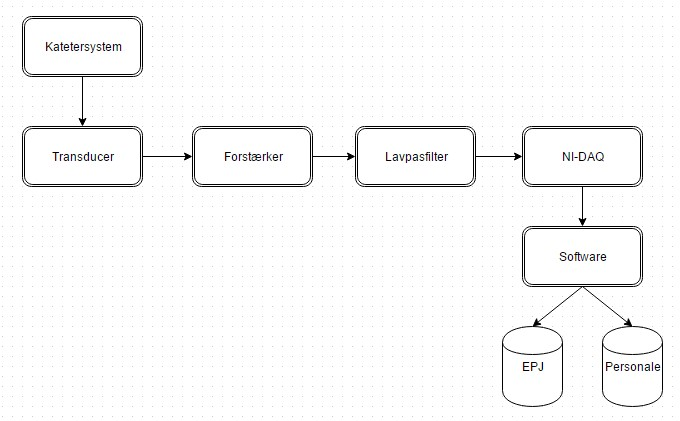
\includegraphics[width =0.8\textwidth , center]{billeder/system}
\caption{\textbf{Skitse af opbygning af systemet.}}
\end{figure}
\chapter{Krav}
Hvilke krav der stilles til produktet, udarbejdes i en kravspecifikation. Denne kravspecifikation består af en række Use cases. Disse Use cases beskriver interaktionen mellem aktørerne og systemet. Use cases har til formål at specificere, hvilke krav der, stilles til produktet. Kravene opstilles ud fra, hvad kunden ønsker, samt hvad leverandøren finder muligt at realisere. \\ \\
Der er nogle obligatoriske krav til produktet, der skal opfyldes. Disse krav er bl.a, at systemet skal kunne kalibrere det indhentede blodtrykssignal og foretage en nulpunkts justering. Desuden skal blodtrykssignalet vises kontinuerligt, hvilket betyder, at signalet skal vises grafisk, samtidigt med at det bliver hentet/indsendt data fra hardwaren. Disse behandlede data skal desuden gemmes i en database.
Et af de obligatoriske krav er desuden, at der skal være et digitalt filter, der kan slås til og fra når programmet kører. Dette filter skal sørge for, at signalet haves i to forskellige modes; et diagnose mode, hvor signalet er råt med alle udsving, og et monitor mode, hvor signalet er filtreret og afrundet.\\\\
Foruden disse obligatoriske krav er det valgt, at det skal være muligt at starte og stoppe målingen. Når målingen er startet skal det være muligt at justere grænseværdierne for systolen og diastolen, så grænseværdierne kan tilpasses patienten. Når signalets værdier overskrider en af grænseværdierne, skal en alarmering begynde. Denne alarm skal kunne udsættes i et minut, dog kun alarmens lyd, så det stadig er tydeligt at se, at en grænseværdi er overskredet.\\
Systemet består af en computer med en programkode, en NI-DAQ, et lavpas filter, en forstærker, en transducer og en In vitro maskine.\\
Blodtrykket dannes i denne prototype af en In vitro maskine, som leverer et tryk til en tryktransducer, herefter sender tryktransduceren signalet videre til hardwaren, hvor signalet bliver forstærket og høje frekvenser bliver dæmpet. Dette signal sendes derefter igennem NI-DAQ ind til softwaren, som derefter behandler og analyserer signalet.\\
Den fulde beskrivelse af de udarbejdede Use cases (fully dressed Use case skema) findes i Projektdokumentationen under Kravspecifikation.
\begin{figure}[H]
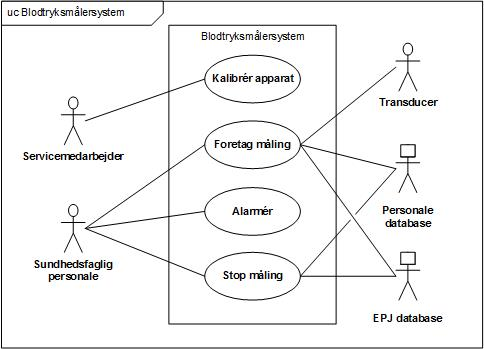
\includegraphics[width =0.7\textwidth , center]{billeder/UseCaseDiagram}
\caption{Use Case diagram. Dette diagram viser aktørernes interaktion med systemet.}
\end{figure}
\section{Aktørbeskrivelse}
Ud fra use case diagrammet ses de seks aktører; \textit{Sundhedsfaglig personale}, \textit{Transducer}, \textit{EKG patient}, \textit{EPJ database}, \textit{Personale database} og \textit{Servicemedarbejder}. Det er disse aktører der interagerer med systemet.
\subsection{Sundhedsfaglig personale}
Det er det sundhedsfaglige personale, der påsætter måleudstyret på patienten. Det sundhedsfaglige personale er desuden den aktør der interagerer med systemet; logger på og foretager en måling. Det sundhedsfaglige personale har dermed adgang til systemet og de viste målinger på brugergrænsefladen.
\subsection{Transducer}
Transduceren agerer som patienten, denne består af en In vitro maskine tilsluttet katetersystemet. Katetersystemet leverer et tryk i mmHg videre til tryktransduceren, som omdanner trykket til et analogt signal. Dette signal sendes videre i hardwaren, som består af en forstærker og et lavpasfilter, som behandler signalet. Signalet behandles i NI-DAQ'en som sendes ind i systemet. Derfor er denne aktør kilden til måleresultaterne for systole, diastole og middeltryk.
\subsection{EKG-patient}
EKG patienten er kilden til EKG-kurven, da der ikke haves en rigtig patient, hvorfra både EKG og blodtryk kan indhentes.\\
Værdierne for denne aktør hentes fra PhysioBank ATM.
\subsection{Servicemedarbejder}
Servicemedarbejderen står for at foretage kalibreringen. Dette gør Servicemedarbejderen ved at koble systemet til kalibreringssystemet, og indtaste de værdier for tryk (mmHg) og spænding (Volt), som kan måles ved tre forskellige målepunkter på en vandsøjle. Herefter kan en kalibreringsværdi findes af systemet.
\subsection{EPJ database}
I EPJ databasen gemme patient- og måledata. Blodtrykskurvens rådata gemmes som en talliste. For at have nok information om signalet gemmes kalibrerings- og nulpunktsjusteringsværdien for signalet også i EPJ databasen. Patienterne i denne database kobles sammen med en sundhedsfaglig person fra Personale databasen. 
\subsection{Personale database}
Det sundhedsfaglige personales login-informationer ligger i Personale databasen. 
\section{Use case beskrivelse}
Use case diagrammet viser ligeledes de fire Use cases, der er for systemet: Kalibrér apparat, Foretag måling, Alamér og Stop måling. Disse Use cases er en beskrivelse af, hvad systemet skal kunne, og beskriver de interaktioner, der sker mellem aktørerne og systemet.
\\
\subsection{Use case 1: Kalibrér apparat}
Servicemedarbejderen skal i denne Use case foretage en kalibrering. Dette gøres ved at der er tre målepunkter på en væskesøjle, hvor én af disse målepunkter vælges. Fra målepunktet måles spændingen (volt), med et multimeter eller Analog Discovery, og trykket (mmHg) aflæses fra væskesøjlen. Disse indtastes af Servicemedarbejderen ind i systemet igennem brugergrænsefladen; startskærmen. Herefter beregner systemet en kalibrerings værdi. Denne værdi bruges til at omskrive de indlæste værdier fra DAQ, til en blodtrykskurve i mmHg.
\subsection{Use case 2: Foretag måling}
Denne Use case indhenter data og præsentere disse. For at dette kan gøres, skal det Sundhedsfaglige personale først logge på systemet. Dette gør aktøren ved at indtaste brugernavn og adgangskode på brugergrænsefladen; startskærmen. Når den sundhedsfaglige er logget på, henter systemet de tilknyttede patienter, hvorefter det Sundhedsfaglige personale kan vælge den ønskede patient. Når Patienten er blevet valgt startes hovedskærmen. \\
For at sikre at graferne, der hentes ligger rigtigt på graferne, skal det Sundhedsfaglige personale nulpunktsjustere systemet, sådan at graferne kommer til at ligge rigtigt på akserne. Dette gøres ved, at der tages højde for det atmosfæriske tryk.\\
Herefter kan den Sundhedsfaglige starte målingen. Når dette gøres, henter systemet blodtrykssignalet og EKG-signalet. Disse bruges af systemet til at beregne systole, diastole, middeltryk og puls. Systemet viser graferne kontinuert på hver sin graf og systole, diastole, middeltryk og puls vises som talværdier. Samtidig gemmer systemet løbende disse data i EPJ databasen. \\
Det vil være muligt for det Sundhedsfaglige personale at slå det digitale filter fra og til. Filteret er pr. default slået til fra start.\\
Det er også muligt for det Sundhedsfaglige personale at justere grænseværdierne for systolen og diastolen, dette gøres for at indstille grænseværdierne individuelt for hver patient.
\subsection{Use case 3: Alarmér}
Alarmen startes af systemet, når en af grænseværdierne for systole eller diastole overskrides. Dette gør at knappen, der benyttes til at udsætte alarmen, blinker skiftevis mellem at have rød og hvid baggrund, og der starter en alarm lyd. Når alarmen er igangsat kan endnu en grænseværdi overskrides, hvis dette sker, er der umiddelbart ikke nogen ændring. Alarmlyden fortsætter fra tidligere, og knappen, til udsættelse af alarmen, fortsætter med at blinke. \\
Det vil her være muligt for det sundhedsfaglige personale af udsætte alarmen. Dette gøres ved at trykke på "Udsæt alarm" knappen, som illustreres med et alarm billede, hvorefter systemet stopper alarmens lyd i et minut. Efter dette minut starter alarmens lyd igen. "Udsæt alarm" knappen fortsætter med at blinke, indtil forholdene er normaliseret, altså indtil grænseværdien ikke længere er overskredet.
\subsection{Use case 4: Stop måling}
Det Sundhedsfaglige personale skal også kunne stoppe målingen. Dette gøres ved, at det sundhedsfaglige personale interagerer med hovedskærmen. Herefter vil det være muligt for det Sundhedsfaglige personale at logge ud, og et nyt scenarie kan påbegyndes.
\section{Ikke-funktionelle krav}
Ikke funktionelle krav er opsat efter FURPS+ metoden. Kravene er herefter blevet prioriteret efter MoSCoW. De udspecificerede ikke-funktionelle krav kan findes i Projektdokumentationen under Kravspecifikationen.
\subsection{FURPS+}
\textbf{Functionality}\\
Funktionalitet er det brugeren ønsker sig. Dette omfatter også sikkerhedsrelaterede behov. Dette er krav til hvad programmet skal kunne af funktionalitet, f.eks. at programmet skal gemme data løbende i en database.\\\\
\textbf{Usability}\\
Hvor effektiv er produktet, set fra forbrugerens side, dette er det aspekt brugervenlighed ser på. Er produktet nemt at bruge. Hvordan bruges produktet; er der nogen brugergrænseflader. Det er herunder kravene til hvilke knapper der skal være på brugergrænsefladerne, og dermed også hvilke brugergrænseflader der skal være.\\\\
\textbf{Reliability}\\
Pålidelighed tager sig af aspekter som, hvor længe er det maksimalt at systemet må være nede. Er der fejl der kan forudses. Hvor præcist kan resultaterne vises. Er produktet let at vedligeholde; kan delene i produktet skiftes let.\\\\
\textbf{Performance}\\
Præstationen for produktet, handler om hvor hurtigt produktet er om at starte op og hvor hurtigt svartiden er. Hvor stor må svartiden maksimalt være. Så det er altså herunder, at det er beskrevet, hvor lang tid der går fra der er trykket på en knap, til at systemet svarer. \\\\
\textbf{S}uportability\\
Produktets support fortæller, om det er muligt at teste på produktet, om det er muligt at udvide produktet, installere og konfigurere produktet. Desuden om produktet er kompatibelt. Det er herunder programmets opbygning beskrives\\\\
\textbf{+}\\
Kunden kan have nogle yderligere behov, disse yderligere behov beskrives under +. Hvilke begrænsninger er der ved designet. Er der nogle krav for brugergrænsefladerne. Er der nogle fysiske eller implementeringskrav. Er der dele der kan genbruges, herunder hele systemer eller dele af dem. Det er bl.a herunder at kravene til computeren, der benyttes, beskrives. \cite{furps}\\
\subsection{MoSCoW}
\textbf{Must}\\
De krav der bliver markeret som et must er de krav som produktet skal have. Altså det produktet skal have/indeholde.\\\\
\textbf{Should}\\
De krav der markeres som et should-krav, er de krav til produktet der burde være med. Altså er det hvad produktet bør indeholde\\\\
\textbf{Could}\\
Kravene kan også markeres som could. Disse krav er de krav der kunne være gode at have med, men som ikke bliver prioriteret højt. Så det er kun, hvis man kan nå at få det med, at de skal være der.\\\\
\textbf{Would/Won't}\\
Det er ikke alle krav, der skal være gældende for produktet, disse krav markeres som would/won't. Det er altså disse krav som man ikke tager med eller de krav som ville være sjove at have med, men ikke har en betydning for produktet, men er en tilføjelse eller udvidelse. Det er disse krav der danner rammen for fremtidigt og videregående arbejde med projektet.
\chapter{Projektbeskrivelse}
\section{Projektgennemførelse}
\subsection{ASE-modellen}
Til udviklingen af dette produkt er der primært benyttet ASE-modellen. Modellen ses herunder. ASE-modellen er en udviklingsmodel, der er udarbejdet af Aarhus Ingeniørhøjskole. Denne model er en mellemvægtig semi-iterativ udviklingsproces, hvilken drives ud fra Use cases. Projektudviklerne fastlægger først en projektformulering, hvorfra en kravspecifikation kan udarbejdes, hvilken indeholder kravene fra kunden. Systemarkitekturen fastlægges ud fra kravspecifikationen, for derefter at designe og implementere de enkelte hardware og software dele hver for sig i iterationer. Til sidst fører dette til en accepttest, hvilken gennemføres, så der opstår en enighed mellem projektudviklerne og kunden.
\begin{figure}[H]
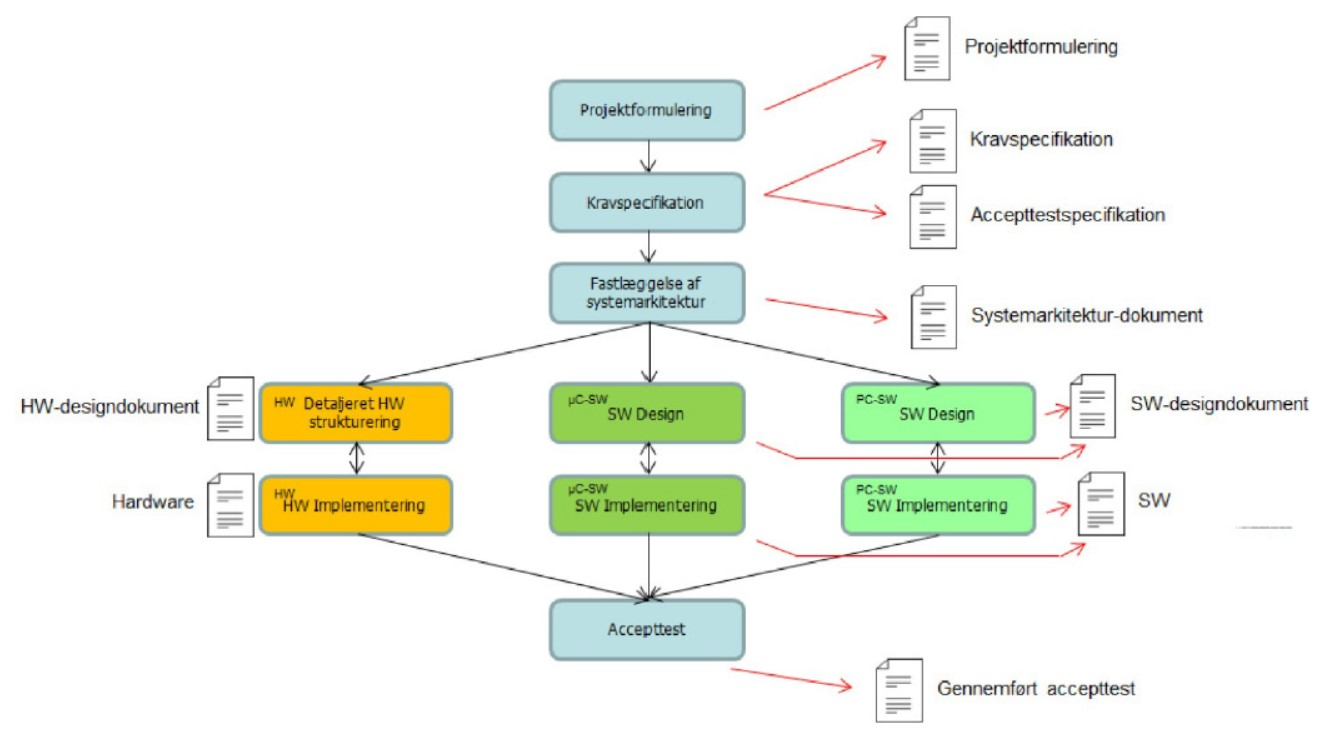
\includegraphics[width =1.0\textwidth , center]{billeder/ASEmodellen}
\caption{ASE-modellen.}
\end{figure} 
Kravspecifikationen bliver specificeret som en række Use cases ud fra problemformuleringen. Use cases benyttes til at beskrive aktørernes interaktion med systemet. Sammen med de ikke-funktionelle krav opnås der med Use casene et overblik over hvilke krav der stilles til systemets funktionalitet. Systemets design bestemmes igennem hardware og software design og implementering, herefter kan en accepttest udarbejdes. Ved udførelsen af accepttesten tjekkes det at kravene er opnået.
\subsection{V-modellen}
V-modellen er en faseopdelt udviklingsmodel. Denne model beskriver udviklingsfaserne og testfaserne i et projekt sideløbende. V-modellem er blevet benyttet sideløbende med ASE-modellen. Specifikationen af test foregår parallelt med udviklingen af selve systemet i V-modellen. Fordelen ved denne model er at testene sker på forskellige niveauer, hvilket sikre at udviklede delsystemer virker som ønsket. Det vigtige her er at en fase er færdiggjort, inden den næste fase påbegyndes. 
\begin{figure}[H]
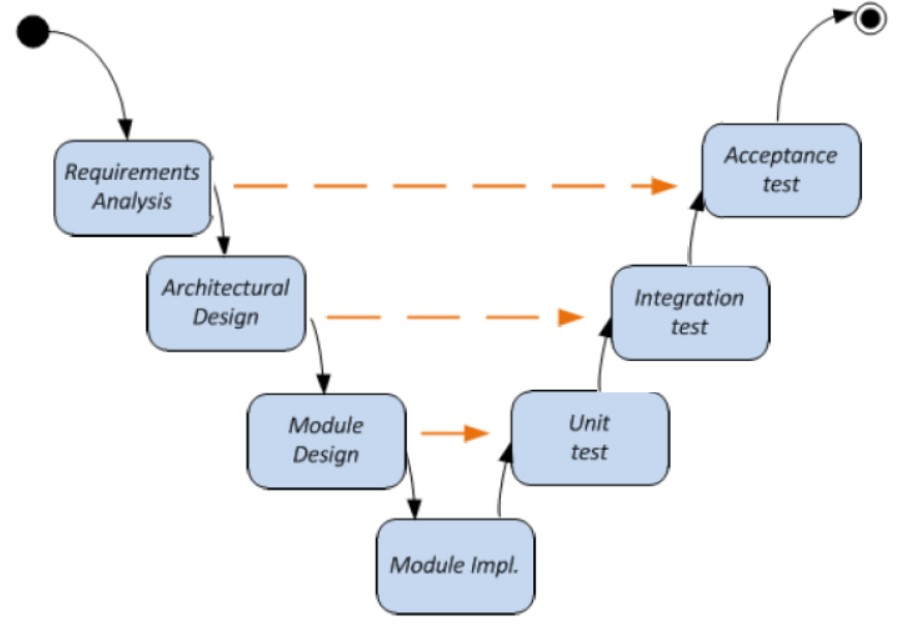
\includegraphics[width =0.7\textwidth , center]{billeder/Vmodel}
\caption{V-modellen.}
\end{figure} 
Ud fra modellen ses det at den første fase er udviklingen af kravspecifikationen. Her udarbejdes der en tilhørende accepttest, denne test gør det muligt at tjekke om systemet til sidst lever op til de opstillede krav. Den næste fase er herefter systemarkitektur, her udvikles den tilhørende test, denne test undersøger integrationen mellem de implementerede moduler. De sidste to fase af udviklingsfasen er design og implementering af systemets enkelte moduler, her udføres enhedstesten løbende af de implementerede moduler.
\subsection{Vandfaldsmodellen}
Vandfaldsmodellen er en model der bruges til udvikling af software og hardware, hvor software- og hardwareudviklingen betragtes som værende konstant nedadløbende. Her kan udviklingen af et modul i en ny fase først påbegyndes når den foranliggende fase er afsluttet. Denne model er i projektet benyttet til udviklingen af software- og hardwarearkitekturen. 
\begin{figure}[H]
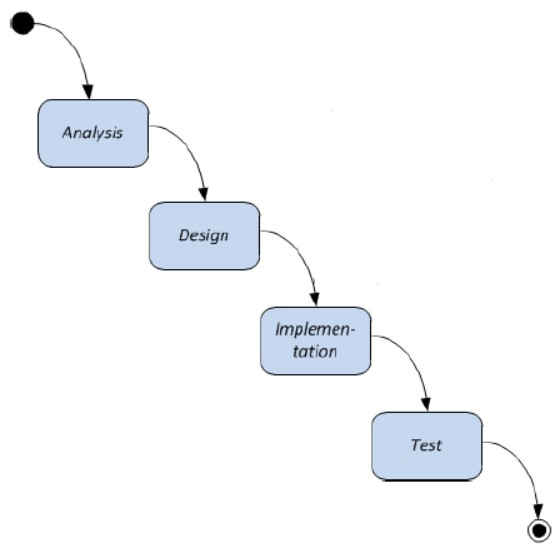
\includegraphics[width =0.5\textwidth , center]{billeder/Vandfald}
\caption{Vandfalds modellen.}
\end{figure} 
Disse tre modeller; ASE-modellen, V-modellen og vandfalds-modellen arbejder alle i en kronologisk logisk rækkefølge. Modellerne er benyttet i et omfang, hvor de har kunnet supplere hinanden. ASE-modellen giver det store overblik, mens V-modellen sikre udarbejdelsen af de nødvendige tests. Vandfalds-modellen er den proces, hvilken der er arbejdet ud fra i alle projektets facetter.   
\subsection{Projektstyring}
\subsubsection{Arbejdsfordeling}
Som nævnt tidligere valgte man fra projektets start at opdele gruppen i to hold, henholdsvis et softwarehold og et hardwarehold.
\subsubsection{Ændringer i projektstyring}
Under projektforløbet blev det valgt at ændre denne rollefordeling, idet den generelle arbejdsfordeling samt arbejdsindsats i projektgruppen ikke fungerede optimalt. Det blev valgt, at kun et gruppemedlem skulle varetage rollen som projektleder og procesleder, men at opgaverne herunder kunne uddelegeres hvis nødvendigt. Denne leder blev i fællesskab valgt og baggrunden for dette, var et ønske om en leder, som både havde viden og indflydelse på hardware og software. Denne leder skulle gribe ind, hvis gruppearbejdet og deltagernes indsat ikke opfyldte den forventningsafstemning, som står skrevet i samarbejdskontrakten. 
\subsubsection{Scrum}
Det blev i øvrigt besluttet at benytte SCRUM som hjælp til styring af projektet. Der blev udnævnt en tovholder, som skulle holde møder i løbet projektets udarbejdelse, samt styre opgaverne. Man valgte at bruge Pivotal Tracker \cite{tracker}  til at styre og prioritere opgaver. Der var en overordnet tidsplan fra start, denne tidsplan består af en række deadlines, som kan findes i Produktdokumentationen.
\subsubsection{GitHub}
Det blev besluttet at benytte GitHub til deling af informationer og dokumentation i forbindelse med udarbejdelse af rapporten. Det blev vurderet, at det var vigtigt, at der var en central informationsudveksling, så begge grupper kunne følge med i, hvor langt de var i de forskellige processer. 
\subsubsection{Iterativ udviklingsproces}
Udviklingsprocessen på både software- og hardwareholdet blev meget iterativ, det betød at der var mange forskellige versioner af både hardware og software. Man valgte denne metode da store dele af projektet var et teknologistudie, så det var nødvendigt at lave mange iterationer løbende. Desuden var det vigtigt, at de to hold kunne omstille sig hurtigt, og bruge ny viden uden at skulle igennem en langsommelig design proces på ny.
\section{Metode}
\cite{SysML} For at beskrive den overordnede systemarkitektur og det detaljerede design for produktet, er der blevet benyttet SysML og UML. SysML er et grafisk modelleringssprog, hvilket kan hjælpe til at forstå og udvikle komplekse systemer. SysML udspringer af UML, dog benyttes SysML i højere grad ved systemer, der både indeholder software og hardware. UML benyttes til at beskrive softwaresystemets struktur og forløb. \cite{uml}
\\
\\
SysML’s struktur-, funktionalitets- og adfærdsdiagrammer er i projektet blevet benyttet til at specificere og dokumentere systemet og dets komponenter. Der anvendes to strukturdiagrammer; block definition diagram (BDD) og internal block definition diagram (IBD) for at vise systemstrukturen. Systemarkitekturen bliver delt op i blokke. BDD'et bruges til at vise forholdet mellem de forskellige blokke, deres komposition og forholdet mellem logiske- og fysiske enheder i systemet. IBD'et benyttes til at vise den forbindelse der er imellem de forskellige blokke der ses ud fra BDD'et. Dermed ses den vej signalet går igennem de forskellige enheder og hvordan disse enheder er koblet sammen.\\
\\ 
For at kunne beskrive produktets funktionalitet, er der blevet udarbejdet et Use case diagram. Dette diagram beskriver, hvordan systemet interagerer med de udefrakommende enheder (f.eks. aktører) for at løse et antal opsatte opgaver. Disse opgaver er beskrevet i forskellige Use cases. \\
Domænemodellen beskriver det overordnede systemdomæne. Systemdomænet beskrives ud fra de konceptuelle klasser, hvilke findes ud fra Use cases. Domænemodellen definerer de klasser, der skal være i softwaren og de interaktioner der er imellem disse, dette gøres med klassediagrammer og adfærdsdiagrammer.\\
Et af adfærdsdiagrammerne er et sekvensdiagram, denne viser de handlinger, der er mellem systemets dele (parts), hvilke er delt op i sekvenser.\\
For at beskrive overgangen fra de beskrevne Use cases til software, er applikationsmodellen benyttet. Applikationsmodellen tager udgangspunkt i Use cases og domænemodellen, hvor Use cases bruges til at identificere, hvad systemet skal kunne. \\
\\
En applikationsmodel med kontrolklasser, domæneklasser og boundaryklasser kan opbygges. Kontrolklasserne beskriver hvordan data behandles mellem domæne- og boundaryklasserne. Domæneklasserne indeholder funktionaliteten som det pågældende softwaremodul benytter, det er herfra klasserne, der skal bruges i softwaren identificeres. Boundaryklasserne har den funktion at beskrive, hvordan systemet kommunikerer med omverdenen og omvendt. Ved at benytte applikationsmodellen til design af softwarens opbygning, gøres det lettere at udvikle et produkt med lav kobling samt høj samhørighed. \\
\\
Systemets softwarestruktur og forløb beskrives ved at benytte UML klassediagrammer. Klassediagrammet definerer relationerne mellem de forskellige klasser. Derfor dannes der et hurtigt overblik over sammenhængen i systemet ved at benytte klassediagrammet.  
\section{Arkitektur}
\subsection{Hardware}
Systemets hardwarearkitektur beskrives på bagrund af systembeskrivelsen og kravspecifikationen. Ud fra relevante diagrammer, som BDD og IBD, kan hardwarens arkitektur beskrives. Samtlige diagrammer og modeller kan findes i Projektdokumentationen under Arkitektur og design. 
\subsubsection{Problem identifikation}
Først skulle der identificeres hvad produktet skal kunne, og hvordan det skulle virke. Der er i første omgang opstillet krav til hardwaren ud fra kravspecifikationen. De første krav til hardwaren var, at hardwaredelen skulle bestå af en forstærker og et lavpasfilter. Der blev i første omgang arbejdet med et lavpasfilter, som ikke var aktivt. Denne idé blev kasseret, da der efter senere overvejelser blev opdaget at lavpasfilteret skulle være et aktivt anden ordens filter af typen Sallen-key. Herved blev kredsløbet for hardwaren opbygget efter en operationsforstærker og et anden ordens lavpasfilter. Da filteret er aktivt, er der tilsat en spændingsforsyning i form af to 9 V batterier. \\
Hardwaren er herved yderligere specificeret igennem udformningen af diagrammerne BDD og IBD. Diagrammerne beskriver, hvilke blokke blodtryksmålesystemet er bygget op af, og signalets vej igennem blokkene.
\subsubsection{BDD - block definition diagram}
Ud fra Use cases og kravene til hardware omkring blodtryksmålesystemet, er der identificeret, hvilke blokke blodtryksmålesystemet består af. Det er identificeret og beskrevet, hvordan hver blok i blodtryksmålesystemet interagerer, og det er indført på BDD’et som stregerne imellem blokken. Der er angivet, hvilke signaler blokkene sender ud imellem hinanden.  
\begin{figure}[H]
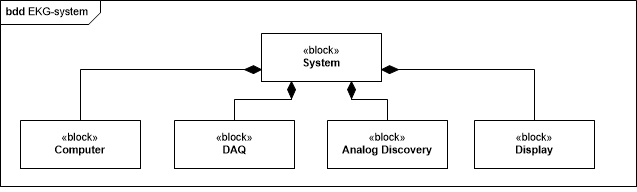
\includegraphics[width =1.0\textwidth , center]{billeder/BDD}
\caption{\textbf{BDD for blodtryksmålesystemet.}}
\end{figure}
Ud fra diagrammet ses det, at alle blokkene er koblet til blodtryksmålesystemet, som er selve softwaren for blodtryksmåleren. Kompositionen i diagrammet viser, at blodtryksmålesystem består af en computer, en transducer, en NI-DAQ, et lavpasfilter, en forstærker og en spændingsforsyning. Disse blokke sørger tilsammen for at forstærke et målt signal og filtrere de høje frekvenser fra. Signalet bliver herefter omformet fra et analog signal til et digitalt signal i NI-DAQ, som blodtryksmåleren indlæser blodtryksdata fra. 
\subsubsection{IBD - internal block definition diagram}
Ud fra block definition diagram kan forbindelserne mellem blokkene identificeres. Dette fører til at et IBD diagram kan opstilles. Et IBD diagram bruges til at vise forbindelserne mellem blokkene, og identificerer hvilke signaler, der sendes ind og ud af hver blok. Det er ud fra et IBD diagram det bestemmes hvilke signaltyper, som blodtryksmålesystemet kan interagere med.
\begin{figure}[H]
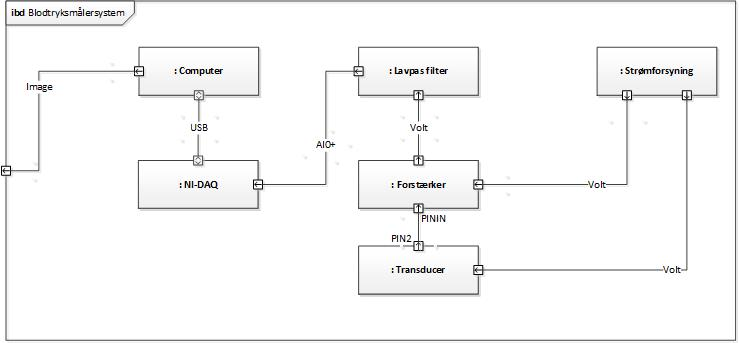
\includegraphics[width =1.0\textwidth , center]{billeder/IBD}
\caption{\textbf{IBD diagram for blodtryksmålesystemet.}}
\end{figure}
\subsection{Software}
Systemets softwarearkitektur beskrives på baggrund af systembeskrivelsen og kravspecifikationen. Ud fra relevante diagrammer og modeller kan softwaren beskrives, hvoraf arkitekturen for softwaren opnås. Samtlige diagrammer og modeller kan findes i Projektdokumentationen under Arkitektur og design.
\subsubsection{Problemidentifikation}
Den første fase i produktudviklingen bestod i, at få klarlagt hvad produktet skulle bruges til og hvilke funktioner dette skulle have. Den første ide som blev udtænkt var en blodtryksmåler, som skulle benyttes til diabetes patienter. Denne ide førte til første udkast af startskærmen. På startskærmen kunne man vælge, hvor på patienten målingen skulle foretages. Her kunne man altså vælge, at blodtryksmålingen skulle foretages invasivt i a. brachialis, samt i underekstremiteterne, og sammenligne disse to. Dette kan klarlægge om blodomløbet i underekstremiteterne er dårligt, da der ses åreforkalkning hos diabetikere. Dog blev denne idé kasseret, idet der med et lavt blodtryk vil være dårlig sårheling og større risiko for infektion.\\\\
Ideen til prototypen blev udtænkt efter samtale med anæstesisygeplejerske Charlotte Høj fra operationsafdelingen på Herning Sygehus. På billedet ses anæstesisygeplejerskens arbejdsfelt, dette består af (fra højre) EPJ system, anæstesi apparat og monitor.
\begin{figure}[H]
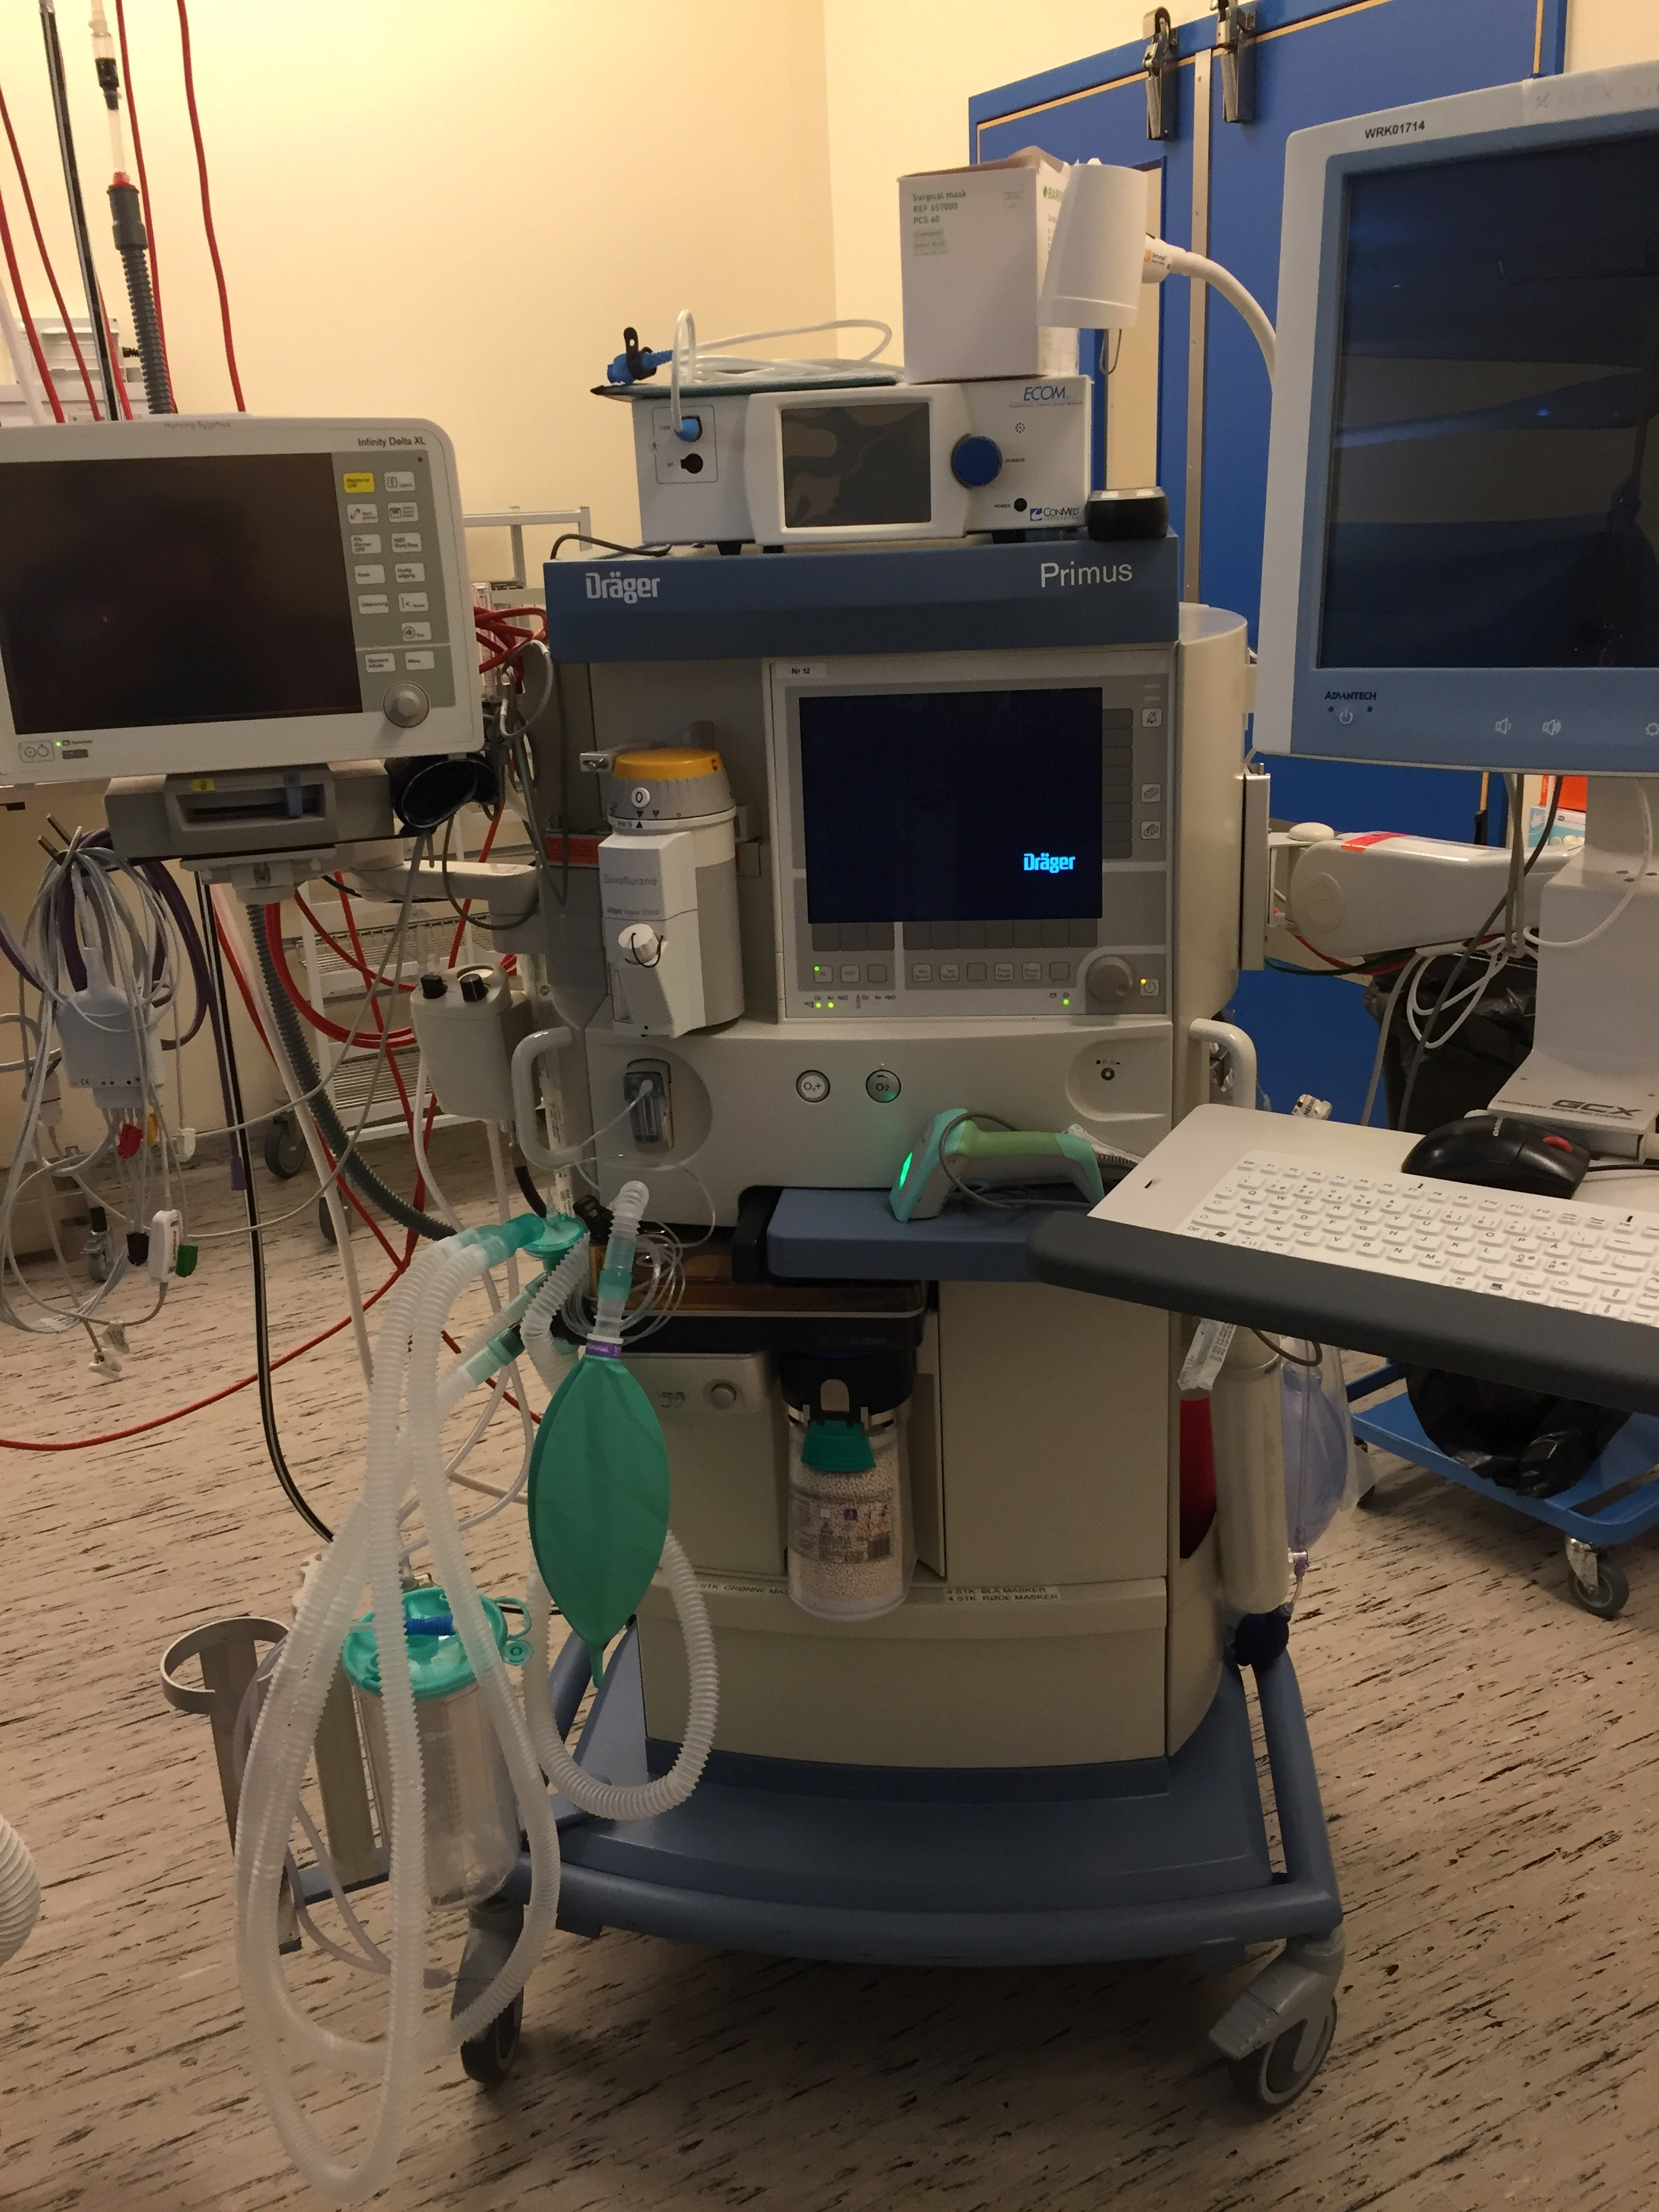
\includegraphics[width =0.4\textwidth , center]{billeder/anastesi}
\caption{\textbf{Anæstesisygeplejerskens arbejdsfelt.}}
\end{figure}
Produktet skulle opbygges med udgangspunkt i et brugsscenarie og efterleve dette arbejdsfelt, dog kun EPJ og monitor, og de hertil tilhørende funktioner. EPJ systemet på Herning sygehus benyttes både til patientjournal og personale login. Det er her sygeplejersken logger på med et unikt bruger-ID og der vil til dette være knyttet de patienter, som hun skal tilgå den pågældende dag. Sygeplejersken vil derfor kunne se relevante data for patienten. Derudover vil det målte blodtryk også gemmes i EPJ systemet. Monitoren er den brugergrænseflade, som grafisk præsenterer blodtrykket, EKG og iltmætning, samt tilhørende værdier. På monitoren er der en start- og slukknap og en timer, som starter når blodtryksmålingen sættes i gang. Derudover er der indbyggede grænseværdier for sysolen og diastolen, som justeres afhængigt af patientens tilstand. 
Ud fra denne idé kunne Use cases udarbejdes, disse er beskrevet under Krav, hvor hovedscenariet for brugen af blodtryksmåleren beskrives.
\subsubsection{Domænemodel} 
Ud fra disse Use cases kunne de klasser som systemet skal bestå af identificeres. Disse klasser identificeres ved at bestemme de konceptuelle klasser, som indeholder den information som systemet skal holde styr på. De konceptuelle klasser indføres i domænemodellen som klasser. Det er i domænemodellen, hvor funktioner i softwaren kan bestemmes. 
\begin{figure}[H]
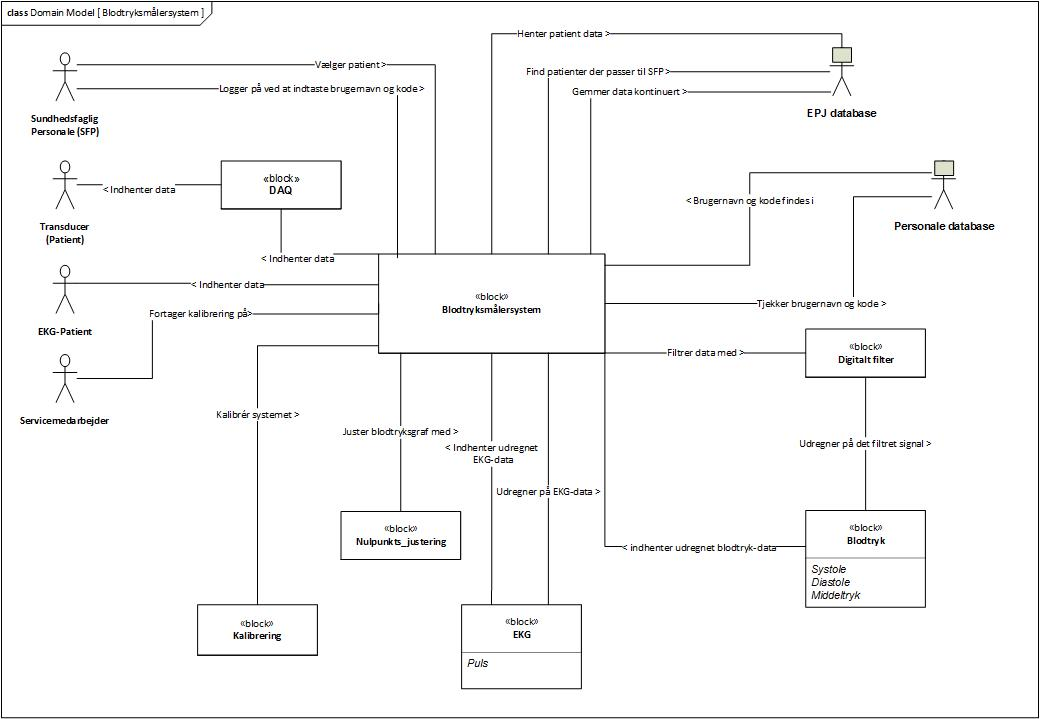
\includegraphics[width =1.0\textwidth , center]{billeder/DM}
\caption{\textbf{Domænemodel for blodtryksmålesystemet.}}
\end{figure}
Ud fra denne model ses det sundhedsfaglige personales interaktion med systemet, samt hvilke handlinger, der igangsættes af denne interaktion. Det sundhedsfaglige personale udfører en handling, der medfører, at en række processer starter i systemet. Disse processer sørger for at hente data fra transduceren og EKG patient, samt sørger for at starte beregningen af værdierne for puls,
systole, diastole og middeltryk. Efter beregningerne viser systemet disse værdier på brugergrænsefladen. 
\subsubsection{Klasseidentifikation}
Ud fra domænemodellen kan softwareklasserne identificeres. Dette medfører, at en applikationsmodel kan opstilles. Applikationsmodellen bruges til at bestemme de interagerende klasser i blodtryksmålesystemet, og hvordan disse klasser interagerer. Det er også ud fra applikationsmodellen, at det kan bestemmes, hvilke klasser der skal ligge i de forskellige lag i trelagsmodellen, da klasserne i applikationsmodellen kan være af typen; domain, boundary og control.\\\\ Controlklasserne er de klasser, der udfører Use casene, ved at interagere med domain- og boundaryklasserne. Boundaryklasserne er de klasser, der repræsenterer aktørerne fra Use Casene og disse aktørers grænseflader. Domainklasserne er de klasser, hvori data bliver behandlet og bearbejdet. Domæneklasserne er de klasser, der skal ligge i logiklaget. Præsentationslaget og datalaget indeholder begge boundaryklasserne, det skal derfor identificeres, hvilke indeholder data og hvilke klasser, hvorfra interaktionerne startes.
\subsubsection{Metodeidentifikation}
Ud fra klasserne identificeret i domænemodellen og applikationsmodellen, kan sekvensdiagrammer laves. Sekvensdiagrammerne er interaktionsdiagrammer og viser derfor, hvordan processerne forløber i forhold til hinanden. Der laves et sekvensdiagram for hver Use case. Ud fra sekvensdiagrammerne kan det altså ses, hvornår og hvordan de forskellige processer forløber i systemet og interagerer med hinanden. Softwaremetoderne kan derfor identificeres ud fra sekvensdiagrammerne. Ud fra sekvensdiagrammerne kan et klassediagram laves. Dette diagram viser hver metode og attribut i hver klasse.\\
Sekvensdiagrammerne og klassediagrammet kan ses i Projektdokumentationen under Arkitektur og design.
\section{Design, implementering og test}
\subsection{Hardware}
\subsubsection{Design}
Fra projektets start var der mange informationer og krav til hardwaren i projektet. Det betød at det ret tidligt blev tydeligt, hvilke delkomponenter hardwaren skulle bestå af. Hardwaren skulle bestå af et lavpasfilter og en forstærker del, samt en spændingsforsyning. Udviklingsprocessen og design af hardwaren skete igennem en række iterationer, disse er nærmere beskrevet i Projektdokumentationen. Dette afsnit vil fokusere på den endelige dimensionering og det endelige design af hardwaredelen.\\\\
\textbf{Lavpasfilter}\\
Det var givet, at det var et aktivt 2. Ordens Butterworth Sallen-key filter, der skulle være lavpasfilter delen i projektet. Det var fra start givet, at der skulle benyttes en OP27 operationsforstærker, ligeledes var en af kondensatorerne givet: C2 = 680nF og R1 = R2. Filteret skulle dimensioneres til en cut-off frekvens på 50Hz, med minimum 20dB dæmpning ved 500Hz. Ud fra disse informationer, samt en kredsløbstegning af filteret kunne der opstilles en overføringsfunktion for kredsløbet:
\begin{align}
T_{v}(s)=\dfrac{V_{out}(s)}{V_{in}(s)}=\dfrac{\dfrac{1}{R1\cdot R2\cdot C1\cdot C2}}{s^2+\dfrac{R1 + R2}{R1\cdot R2\cdot C2}\cdot s+\dfrac{1}{R1\cdot R2\cdot C1\cdot C2}}
\end{align}
Denne overføringsfunktion omskrives til standardformel:
\begin{align}
\dfrac{V_{out}(s)}{V_{in}(s)}=\dfrac{\omega^2}{s^2+2\zeta\omega\cdot s+\omega^2}
\end{align}
Her isoleres cut-off frekvensen ($\omega$) i overføringsfunktionen for lavpasfilteret:
\begin{align}
\omega = 2\pi\sqrt{\dfrac{1}{R1\cdot R2\cdot C1\cdot C2}}
\end{align}
I denne ligning indsættes de kendte værdier. Det er beskrevet at filteret er af typen 2. ordens Sallen-key filter, derfor ved vi at C1 er halvdelen af C2.\cite{wikifilter}
\begin{align}
50Hz\cdot 2\cdot \pi = \sqrt{\dfrac{1}{R\cdot R\cdot 680\cdot 10^{-9}F\cdot 340\cdot 10^{-9}F}}
\end{align}
\begin{align}
R=6,62\cdot 10^3 \Omega
\end{align}
Ud fra dette ses det at modstanden er ca. 6.6k$\Omega$, realiseret med to 3.3k$\Omega$ modstande i serie i det endelige produkt.\\\\
\textbf{Forstærker INA-114 og valg af spændingsforsyning}\\
Udviklingen af forstærkerdelen til hardwaredelen blev bestemt ved hjælp af databladet for DAQ (NI-DAQ6009), samt databladet for tryk-transduceren (TruWave\texttrademark). DAQ kan maksimalt modtage op til +/-10V, det vil sige signalet ikke må overstige peak-to-peak spænding på 20V. Før forstærkningen kunne beregnes, skulle spændingsforsyningen til kredsløbet vælges. Det blev valgt at benytte to 9V-batterier. Disse blev sat op som følger:
\begin{figure}[H]
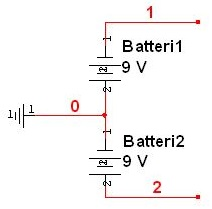
\includegraphics[width =0.2\textwidth , center]{billeder/spandingsforsyning}
\caption{\textbf{Spændingforsyning.}}
\end{figure}
Denne opsætning ville i teorien sikre en 18V peak-to-peak spænding. Det blev valgt at benytte en INA-114 forstærker til at forstærke signalet fra tryktransduceren. I teorien ville man kunne forstærke op til 18V peak-to-peak, men i praksis ville det være urealistisk, da batterierne med tiden bliver afladet. Det blev besluttet at forstærke op til 16V peak-to-peak. Undersøgelser for hvorvidt INA-114 havde tilstrækkelige båndbredde blev udregnet som følger. Først bestemte man det maksimale output for tryktransduceren i området 0-250mmHg.
\begin{align}
V_{max}=250mmHg\cdot 5V\cdot 5\mu V/V/mmHg =6.25 mV
\end{align}
Ud fra dette kan man bestemme hvor meget gain der skal bruges fra forstærkeren.
\begin{align}
16V = 20\cdot 10^{-3}V\cdot gain
\end{align}
\begin{align}
gain = 800
\end{align}
Man sikrede sig at forstærkeren kunne håndtere forstærkningen, denne del er nærmere beskrevet i dokumentationen. Herefter skulle man beregne hvor stor modstanden på INA-114 skulle dimensioneres til for at få den valgte gain.
\begin{align}
G=1+\dfrac{50k\Omega}{R_G}\\
R_G\approx 62.5\Omega
\end{align}
Det blev besluttet at bruge et potentiometer i stedet for en fast modstand til $R_G$. Så man kunne regulere denne hvis spændingsforsyningen var mere potent end 16V peak-to-peak.\\\\
\textbf{Spændingsregulator}\\
Det blev i den sidste iteration besluttet at benytte en spændingsregulator for at sikre at transduceren fik en stabil spændingsforsyning. Tryktransduceren er meget følsom så derfor var det vigtigt at denne får en konstant spændingsforsyning. Det betyder også at den oprindelige skalering ikke er korrekt.
\begin{align}
V_{max}=250mmHg\cdot 16V\cdot5\mu V/V/mmHg =20 mV
\end{align}
Gain beregning
\begin{align}
16V = 6,25\cdot 10^{-3}V\cdot gain
\end{align}
\begin{align}
gain=2560
\end{align}
Produktet af gain og båndbredden er konstant, derfor er det vigtigt båndbredden ligger over knækfrekvensen på 50Hz. Ved gain=1 kan INA-114 levere 1Mhz båndbredde. Følgende ligning for beregning af båndbredden kan opstilling:
\begin{align}
1000000=2560\cdot BW\\
BW\approx 390Hz
\end{align}
Da 390 Hz er over knækfrekvensen på 50Hz har forstærkeren tilstrækkelig båndbredde. Den nye $R_G$ kan beregnes til at skulle være.
\begin{align}
2560=1+\dfrac{50k\Omega}{R_G}\\
R_G\approx 19,5\Omega
\end{align}
\subsubsection{Implementering}
Implementeringsprocessen har været præget af de mange ændringer, som er foretaget undervejs i hardwaredesignet. Disse ændringer er nærmere specificeret i Projektdokumentationen under afsnittet Arkitektur og design for hardware. \\
Hver gang gruppen har identificeret en fejl i hardwaredesignet, som medførte ændringer i kredsløbet, skulle implementeringen af systemet også ændres. Implementeringsstrategien bestod af to faser. Den første fase var at realiserer kredsløbet på et fumlebræt, således at fejl i systemet nemt kan ændres uden store tidsomkostninger. \\\\
Når denne fase er gennemført, skulle systemet overføres på et print som skulle designes vha. Multisims Ultiboard. Gruppens medlemmer havde ikke en forudgående erfaringer med at designe print i Ultiboard. Der er lagt en del tid i at færdiggøre printet, men undervejs i processen, har gruppen valgt at prioritere den første strategi, eftersom tidsforbruget på at designe printet blev for stort. \\
Efter færdiggørelsen af det endegyldige design blev elektronikkredsløbet bygget på et fumlebræt og testen af kredsløbet blev igangsat. Der er anvendt Analog Discovery til simulering af signalet fra transduceren. Dette gøres ved at genererer et differentielt signal fra Analog Discovery, hvor W1 og W2 skal tilkobles til de to indgange på INA-114. De to signaler har samme stelpunkt. Udgangssignalet måles vha. et oscilloskop. De to signaler fra henholdsvis W1 og W1 var på 20mV med forskellige frekvenser. Det forventet resultat er at de 20mV bliver forstærket og ved frekvensen 500Hz skal signalet dæmpes med 20dB. Inden accepttesten skulle eksekveres blev kredsløbet overført på et veroboard for at overskueliggøre kredsløbet. Denne beslutning var ikke en del af den oprindelige plan, eftersom gruppen havde tiltro til ar færdiggøre et print i Ultiboard til tiden. Resultatet af simuleringen og accepttestens udførelse vil blive fremlagt i afsnittet Resultater og diskussion. 
\subsubsection{Modultest}
Modultesten omfatter en forstærkerdel og en filterdel. De udleverede dele af systemet består af en transducer, et kateter og en dataopsamler i form af NI-DAQ-6009. Ved test af filteret sikres det at de høje frekvenser dæmpes. Modultesten foretages enkeltvis, dvs. de enkelte blokke testes hver for sig. Til sidst testes systemet med en vandsøjle for at identificere om forstærkeren og filteret kommunikere med hinanden. Rækkefølgen som blokkene skal testes er som følgende:
\begin{itemize}
\item Test af forstærker
\item Test af filter
\item Den endelige test med vandsøjle
\end{itemize}
Modultesten er nærmere beskrevet i Projektdokumentationen under Arkitektur og design.
\subsection{Software}
Ud fra arkitekturen kan designet af softwaren bestemmes. Det bestemmes, hvilke mønstre der skal benyttes og hvordan data skal transporteres igennem koden. Herudover beskrives, hvordan nulpunktsjusteringen og kalibreringen foretages.
\subsubsection{Kalibrering}
Kalibreringen er blevet implementeret så der indtastes en værdi for trykket, som vandsøjlen leverer i mmHg, og en værdi for spændingen i volt, hvilken kan aflæses fra waveforms eller måles vha. et multimeter. Disse to værdier bliver herefter sendt ned i software klassen Kalibrering, hvor en kalibreringsværdi/omsætningsværdi kan udregnes ved formlen:
\begin{align}
X\left[\dfrac{mmHg}{V}\right]=\dfrac{pressure \left[mmHg\right]}{voltage \left[V\right]}
\end{align}
Den værdi der her udregnes benyttes herefter til at omregne den spænding i volt, der indsendes i systemet, til tryk i mmHg. 
\begin{align}
voltage \left[V\right]\cdot X\left[\dfrac{mmHg}{V}\right] = pressure \left[mmHg\right]
\end{align}
Hermed ganges kalibreringsværdien på samtlige værdier i den liste af data der kommer fra DAQ'en (Blodtryksværdiliste). 
\subsubsection{Nulpunktsjustering}
Nulpunktsjusteringen foregår ved, at transduceren er tilsluttet og måler det atmosfæriske tryk, denne værdi skal herefter trækkes fra samtlige værdier for blodtrykket fra DAQ'en. Denne værdi skal derfor trækkes fra inden kalibreringsværdien ganges på. Måden hvorpå nulpunktsjusteringen foregår, er ved at transduceren er tilsluttet, og vha. waveforms kan det atmosfæriske tryk aflæses, denne værdi aflæses som en spænding. Denne værdi indtastes på hovedskærmen, hvorefter nulpunktsjusteringen kan startes. Systemet går herefter ind i klassen Nulpunkts$_{-}$justering, hvor følgende formel bruges til at beregne den værdi der skal benyttes videre:
\begin{align}
V_{zero} \left[V\right]=V_{read}\left[V\right]-pressure \left[V\right] 
\end{align}
Det er denne værdi, der herefter bliver kalibreret, for derefter at kunne blive vist som en graf for blodtrykket i mmHg.
\subsubsection{Digitalt filter}
Det digitale filter, der er blevet implementeret i projektet, er af typen et glidende middelværdi (moving average) filter. I et glidende middelværdi filter, lægges der et vindue oven på talværdien, i dette vindue tager man gennemsnittet af alle værdierne. \cite{digifilter} Vinduet er her betegnelsen for et bestemt tidsinterval. \\
I projektet er længden på vinduet valgt til at være ti. Det betyder, at for hvert tiende tal i vores blodtrykliste, bliver gennemsnittet beregnet. Herefter rykker vinduet sig til højre og udregner for de næste ti tal i blodtrykslisten. Blodtrykslisten er listen af blodtryksværdier, der bliver indlæst af DAQ’en. 
\begin{figure}[H]
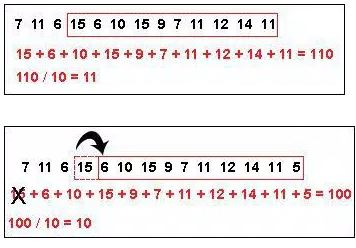
\includegraphics[width =0.5\textwidth , center]{billeder/RammeDigi}
\caption{\textbf{Digital filter ramme. Denne viser hvordan rammen bestemmer gennemsnittet og rykker én hver gang.}}
\end{figure}
Et glidende middelværdi filter kan beskrives med formlen:
\begin{align}
y\left[n\right] = \dfrac{1}{M}\cdot \sum_{k=0}^{M}x\left[n-k\right]
\end{align}
\begin{align}
b_{k}=\dfrac{1}{M}
\end{align}
$M$ er de forgående samples for signalet, $n$ er de nuværende værdier af blodtrykket og $k$ er koefficienterne. 
Filteret udglatter signalets høje peak værdier, da filteret er et lavpasfilter.
\subsubsection{Observer mønsteret}
Observer mønsteret bruges til at sende data op kontinueret. Subject har en metode til at koble en observer til, og en anden metode til at fjerne observeren. Der er en tredje metode i subject, kaldet Notify. Notify sørger for at give besked til den tilknyttede observer om opdatering. En observer er interesseret i at kende til ændringer i det subject den er tilknyttet. Beskeden om ændring kommer fra subjectet, der er tilknyttet observeren. \\
\\
I dette projekt er det valgt at bruge observer mønsteret til at sende data fra datalag til logiklaget. Mønsteret er også brugt til at sende data videre fra logiklaget til præsentationslaget. Yderligere beskrivelse findes i Projektdokumentationen under kapitlet Arkitektur og design under afsnittet Software design. 
\subsubsection{PUSH/PULL}
PUSH/PULL er to forskellige måder at implementere observer mønster på. Her bliver data enten skubbet eller trukket op. PUSH betyder at skubbe, og betyder at data bliver skubbet op, når der sker en ændring, uden der skal gives besked om at hente data. PULL trækker data op imellem lagene. I PULL gives der besked til et lag om en ændring. Herefter skal laget, der ønsker at kende til ændringen bede om ændringen, før det sendes op.\\
\\
I dette projekt er det valgt at benytte PUSH til at sende data imellem lagene. Det er interessant at få data op til brugergrænsefalden hele tiden, når der ny data tilgængelig. Yderligere beskrivelse findes i Projektdokumentationen under kapitlet Arkitektur og design under afsnittet Software design. 
\subsubsection{Queue}
For at sikre, at data bliver sendt op i den rigtige rækkefølge og på en kontrolleret måde, er der i dette projekt valgt at benytte en kø. Til dette er der benyttet en indbygget funktion i .NET, Queue class. Herunder ligger der to metoder, som kan bruges til at sende objekter af tal ind i den ene ende af køen. Efter at køen er blevet fyldt op, er der en funktion til at fjerne det første objekt fra den anden ende af køen. Dette sørger for, at der hele tiden er et flow i køen når der sendes data ind i denne. \\
\\
En yderligere beskrivelse af hvordan Queue klassen benyttes i koden og hvordan denne er opbygget er beskrevet i dokumentationen under Arkitektur og design under afsnittet Implementering.
\subsubsection{Trelagsmodel}
Trelagsmodellen er en software model, til at inddele software i tre lag; præsentationslaget, logiklaget og datalaget. Hvert lag har sit eget ansvar og funktion. Præsentationslaget kan kun tilgå logiklaget, og må kun vise data på brugergrænseflade eller indlæse data fra brugergrænsefladen. Logiklaget må tilgå både datalaget og præsentationslaget. Logiklaget er det midterste lag, og står for behandling af data fra præsentationslaget og datalaget. Datalaget er det nederste lag og sørge for at sende data, fra et måleapparat, op til logiklaget. Datalaget står også for at gemme data i en fil eller en database.\\
\\ 
I dette projekt er koden opdelt efter trelagsmodellen, ved at have et præsentationslag med to brugergrænsefalder, et logiklag med algoritmer til udregning af blodtryk, og et datalag der henter data fra DAQ’en og gemmer dem i en database. Yderligere beskrivelse, og model over trelagsmodellens inddeling af software koden, findes i Projektdokumentationen under kapitlet Arkitektur og design under afsnittet Software design.
\subsubsection{Databaser}
\begin{figure}[H]
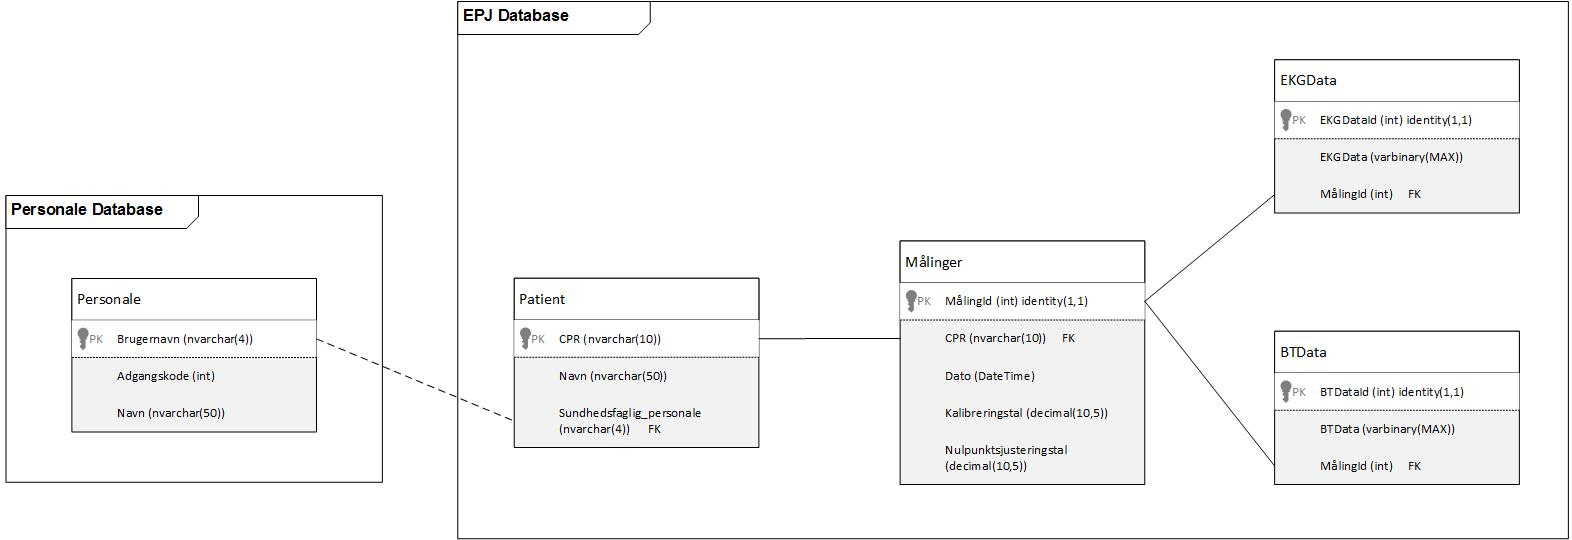
\includegraphics[width =1.0\textwidth , center]{billeder/databaser}
\caption{\textbf{Databaserne; Personale database og EPJ database. Her ses sammenhængen mellem tabellerne i databasen, og hvilken data der er under hver tabel.}}
\end{figure}
Dette afsnit vil beskrive opbygningen af databaser og tabellerne. Da der er valgt at tage udgangspunkt i et brugsscenarie, afspejler datamodelleringen i databasen dette scenarie. Det er vigtigt at bemærke, at der er en regulær opdeling af databaser og skemaer, realiseret som beskrevet nedenfor.
\\\\
\textbf{Personale database}\\
Personale databasen bliver brugt til at tilgå data for personalet. Her er der tale om brugernavn og password. Disse data er lagt i databasen på forhånd, så det er altså en login-database.\\ 
\textbf{Database-adresse:} webhotel10.F15ST2ITS2201404669.db\_ owner
\\\\
\textbf{EPJ database}\\
EPJ databasen bliver brugt til at tilgå data for patienten. Her tænkes på CPR og Navn. Ligeledes gemmes der i denne database målinger, samt metadata for at kvalificere disse målinger. Der kunne udvides med mange flere metadata, specielt i forhold til afsnittet om fremtidigt arbejde "Datawarehouse". Det bør bemærkes, et der i databasen er gjort klar til EKG-data, selvom det ikke er implementeret. Patient-tabellen modsvarer vores version af en EPJ-database, hvor BTData-tabellen repræsenterer målingerne foretaget af vores system.\\
\textbf{Database-adresse:} webhotel10.F15ST2ITS2201405838.db\_ owner. 
\subsubsection{Unittest}
Det er blevet besluttet at lave unittest på softwaren. Unit-test forstås ved, at der testes på hvert enkelt komponent i koden, i objektorienteret kode vil det sige metoderne. Man sikrer sig, at metoderne returnerer det forventede. En unit test bør foregå løbende mens koden bliver udviklet, så man kan fokusere på de del-elementer, som ikke virker efter hensigten. \\
\\
I dette projekt blev der valgt at lave unit-test efter sidste iteration af koden, da de sidste versioner af softwaren ændrede sig meget, så alle unit-tests skulle laves forfra. Grundlaget for mange metoder ændrede sig løbende. Disse unit-tests blev lavet i koden ved at sætte breakpoints og følge metoden til ende og evaluere på hvorvidt metoden opførte sig efter hensigten. Unit-tests er blevet foretaget i koden, hvor der er skrevet kommentarer i koden til de metoder, der er blevet testet.
\section{Resultater og diskussion}
\subsection{Hardware}
Følgende resultater blev foretaget på den næstsidste iteration af hardware-delen. Det betyder at resultaterne ikke er retvisende i forhold til den endelige version af hardwaren. Det har betydning for forstærkningen samt den spænding der fås fra transduceren. \\\\
De vigtigste resultater på hardware delen inkluderer signal forstærkning og signal filtrering. Til simulering af transduceren blev der genereret et signal på 20mV fra Analog Discovery og det forventet resultat var at filtret dæmper frekvenser over 50Hz. De målte målinger fra forstærkeren: 
\\\\
\begin{tabular}{| l | l |} \hline
\textbf{Frekvens [Hz]} & \textbf{Gain. [V] Peak to peak}\\\hline
1 & 16,308 \\\hline 
10 & 17,512 \\\hline
25 & 17,558 \\\hline 
49 & 17,512\\\hline
70 & 17,258\\\hline 
100 & 17,308 \\\hline
250 & 16,278\\\hline
500 & 15.051\\\hline
\end{tabular}\\\\
Som det ses på tabellen har operationsforstærkeren levet op til det forudsete udfald. De 20mV bliver forstærket. Det gain, som er beregnet i teorien var 800 og det målte er i overensstemmelse med det teoretiske gain.  
\begin{align}
output_{INA114}=20\cdot 10^{-3}\cdot 800=16
\end{align}
Den anden måling, som skulle foretages, var for at se om filtret levede op til det krav, der var opstillet, nemlig en cut-off frekvens på 50Hz. Resultatet af denne måling er som følgende:   \\\\
\begin{tabular}{| l | l |} \hline
\textbf{Frekvens [Hz]} & \textbf{Peak to peak [V]}\\\hline
1 & 13,504 \\\hline 
10 & 13,220 \\\hline
25 & 12,412 \\\hline 
49 & 10,644\\\hline
70 & 6,658 \\\hline 
100 & 3,662 \\\hline
250 & 0,666\\\hline
500 & 0,220\\\hline
\end{tabular}\\\\
Om filtret har levet op til det forventet resultat kan tjekkes som følgende:
\begin{align}
G_{dB}=20\cdot log\left(\dfrac{V}{V_{out}}\right)=20\cdot \left(\dfrac{16,308}{0,220V}\right)=-37,234dB
\end{align}
Kravet til filtret var, at ved frekvensen på 500Hz skal signalet dæmpes med minimum 20dB. Overstående beregning giver en dæmpning på 37,234 dB, hvilket opfylder kravet. Ved knækfrekvensen skal dæmpningen være 3dB og det kan regnes som følgende: 
\begin{align}
G_{dB}=20\cdot log\left(\dfrac{V}{V_{out}}\right) = 20\cdot log\left(\dfrac{10,664V}{15,051V}\right)=-3,009dB
\end{align}
Ud fra de overstående beregninger, kan det ses at både forstærkeren og filteret lever tilnærmelsesvis op til kravene. Det skal dog igen nævnes, at det ikke er den sidste iteration af hardwaren, som blev bygget på veroboard med spændingsregulator.
\subsection{Software}
Igennem integrationstesten og accepttesten er der opnået resultater for projektet. Igennem accepttesten er der opstillet krav til hvordan blodtryksmålesystemet skal opføre sig, i forhold til Use cases, og hvordan dette kommer til udtryk visuelt. Resultaterne for projektet er visuelle resultater af accepttesten, og ses i dette afsnit som screendumps. \\\\
I accepttesten er det første step for Use case 1, at vælge en værdi på vandsøjlen og kalibrer efter denne. Herved skal den aflæste spænding og trykket i vandsøjlen indtastes. Når programmet starter, vises startskærmen nedenfor.
\begin{figure}[H]
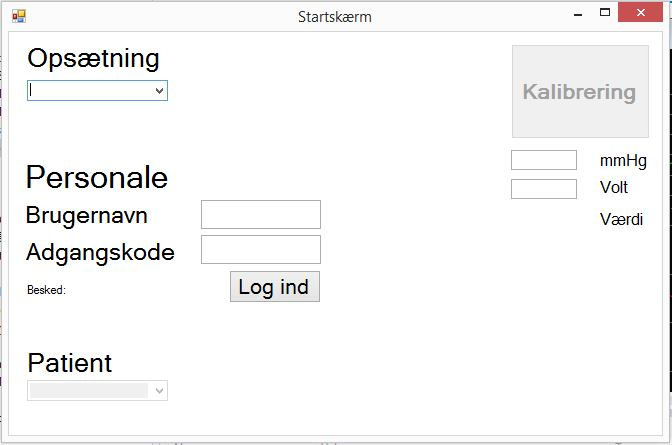
\includegraphics[width =0.4\textwidth , center]{billeder/ITstartGUI}
\caption{\textbf{Startskærm uden indtastede login oplysninger.}}
\end{figure}
Der kan ses på figuren nedenfor, at det er muligt at kalibrere på hovedskærmen, og at blodtryksmålesystemet selv udregner en kalibreringsværdi ud fra de indtastede oplysninger. Kalibreringsværdien udregnes først, når der er trykket på kalibreringsknappen. 
\begin{figure}[H]
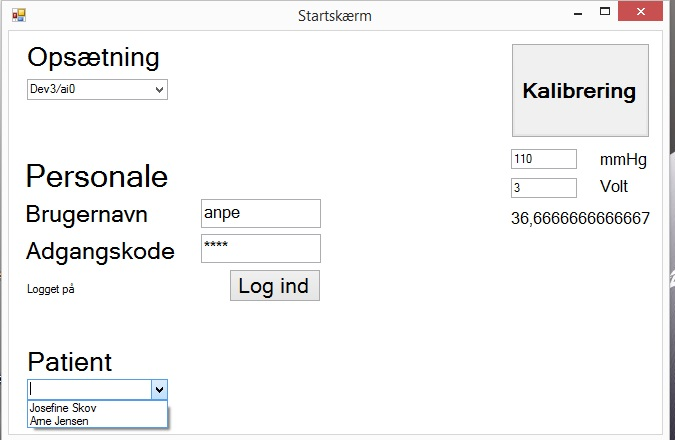
\includegraphics[width =0.4\textwidth , center]{billeder/ITstartGUIlogKali}
\caption{\textbf{Startskærm med login oplysninger og kalibreringsværdi.}}
\end{figure}
Næste step i accepttesten for Use case 2, er at indtaste brugernavnet "anpe" og koden "1234". Derefter trykkes der på login og patienten vælges i patient dropdown. Inden dette er sket, er der valgt den port, som DAQ’en er tilkoblet computeren, og der er forbindelse til VPN. På figuren ovenfor, kan det ses, at der er indskrevet brugernavn og adgangskode for anpe, og der vises hvilke patienter anpe kan tilgå i patient dropdown. Efter at have valgt en patient i patient dropdown, kommer hovedskærmen frem. Her skal der trykkes på tænd-knappen, og derefter bliver grafen for blodtrykket vist, samt værdierne for systolen, diastolen og middeltrykket. Det ses på figuren nedenfor, at blodtrykket bliver vist med filteret på, der vises en systole værdi på 125 mmHg, en diastole værdi på 83 mmHg og et middeltryk på 96 mmHg.
\begin{figure}[H]
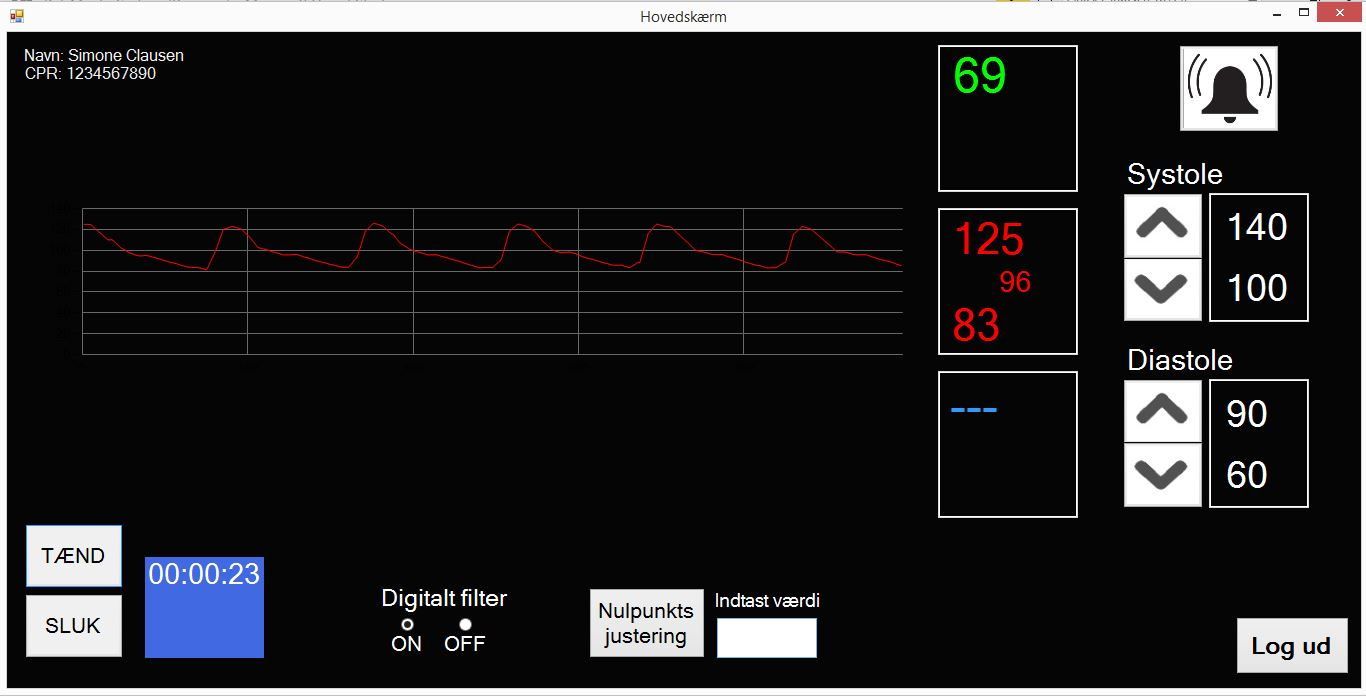
\includegraphics[width =0.6\textwidth , center]{billeder/IThovedGUIkorer}
\caption{\textbf{Blodtryksmåling med det digitale filter slået til.}}
\end{figure}
Blodtryksmålesystemet skal også kunne angive, hvis brugernavnet/adgangskoden ikke findes i databasen. Herved er der i accepttesten for Use case 2, indtastet brugernavnet efgh og koden 1234. Denne kombination findes ikke i personale databasen, og kan herved ikke bruges til at logge ind med. Som det ses på figuren nedenfor, er det heller ikke muligt at logge ind, og programmet giver besked om, at brugernavn og/eller adgangskode er indtastet forkert.
\begin{figure}[H]
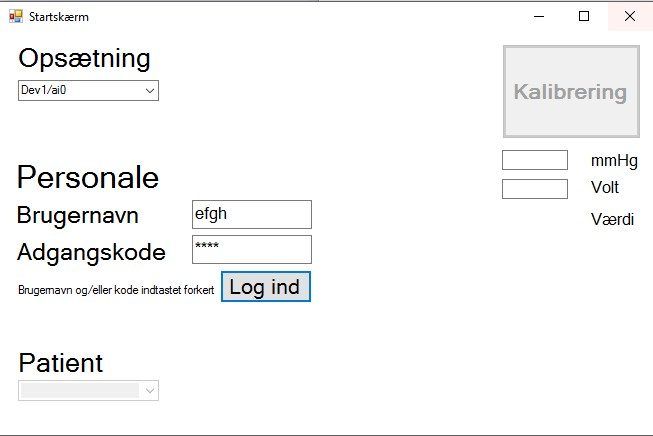
\includegraphics[width =0.4\textwidth , center]{billeder/ITstartGUIforkert}
\caption{\textbf{Brugernenavn/adgangskode er indtastet forkert.}}
\end{figure}
I blodtryksmålesystemet skal det være muligt at kunne slå filteret til og fra, dette bliver testet i accepttesten ved at klikke i radiobutton for digitalt filter off. På figuren nededfor ses det, at blodtrykssignalet er forvrænget, da der er kommet mere støj på signalet, herved kan det konkluderes at filteret virker. 
\begin{figure}[H]
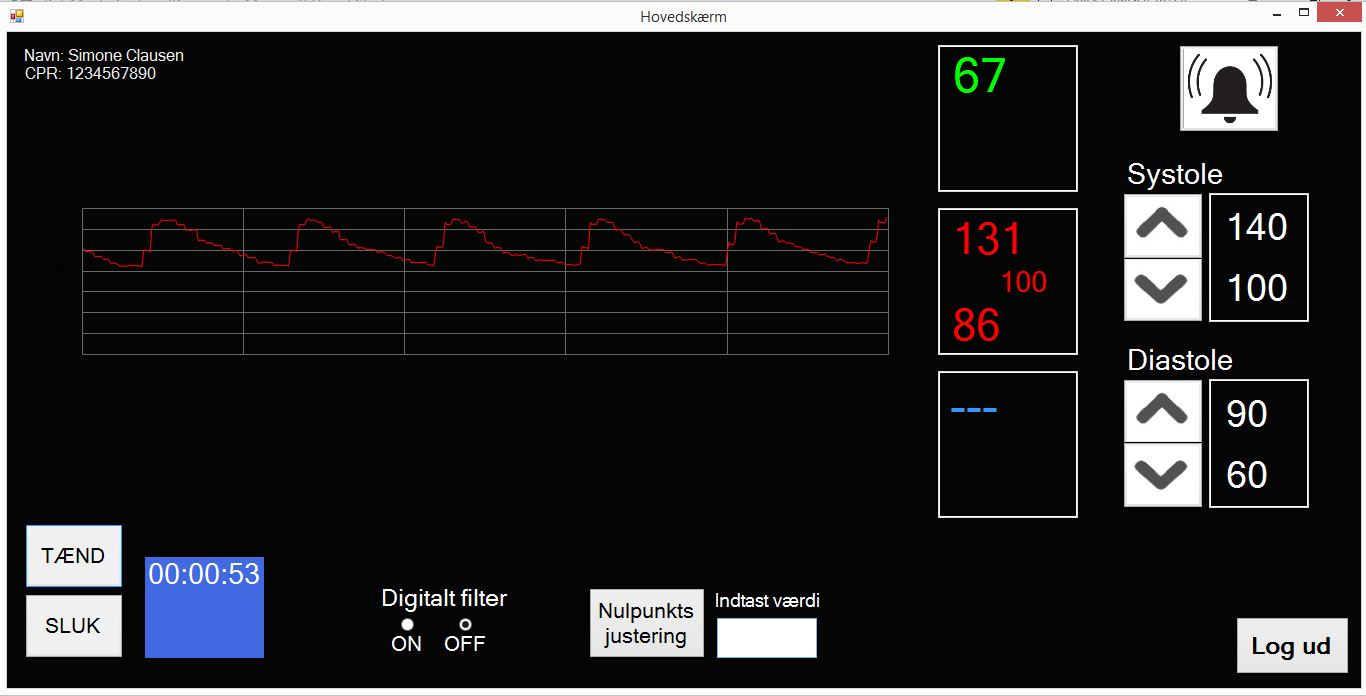
\includegraphics[width =0.6\textwidth , center]{billeder/IThovedGUIkorerufiltreret}
\caption{\textbf{Blodtrykssiganelet uden digitalt filter.}}
\end{figure}
I accepttesten skal blodtryksmålesystemet kunne alarmer når grænseværdierne overskrides, og grænseværdierne skal kunne ændres på hovedskærmen. På figuren nedenfor, ses det at grænseværdierne for systolen op og ned, er ændret til 129/89 mmHg, hvor de før var sat til normal værdierne for systolen; 140/100 mmHg. Blodtrykssignalet har en systoleværdi på 132 mmHg, hvilket er overskrider den nye grænseværdi på 129, og derved går alarmen igang, som det ses med den røde alarm klokke øverst i højre hjørne af hovedskærmen. 
\begin{figure}[H]
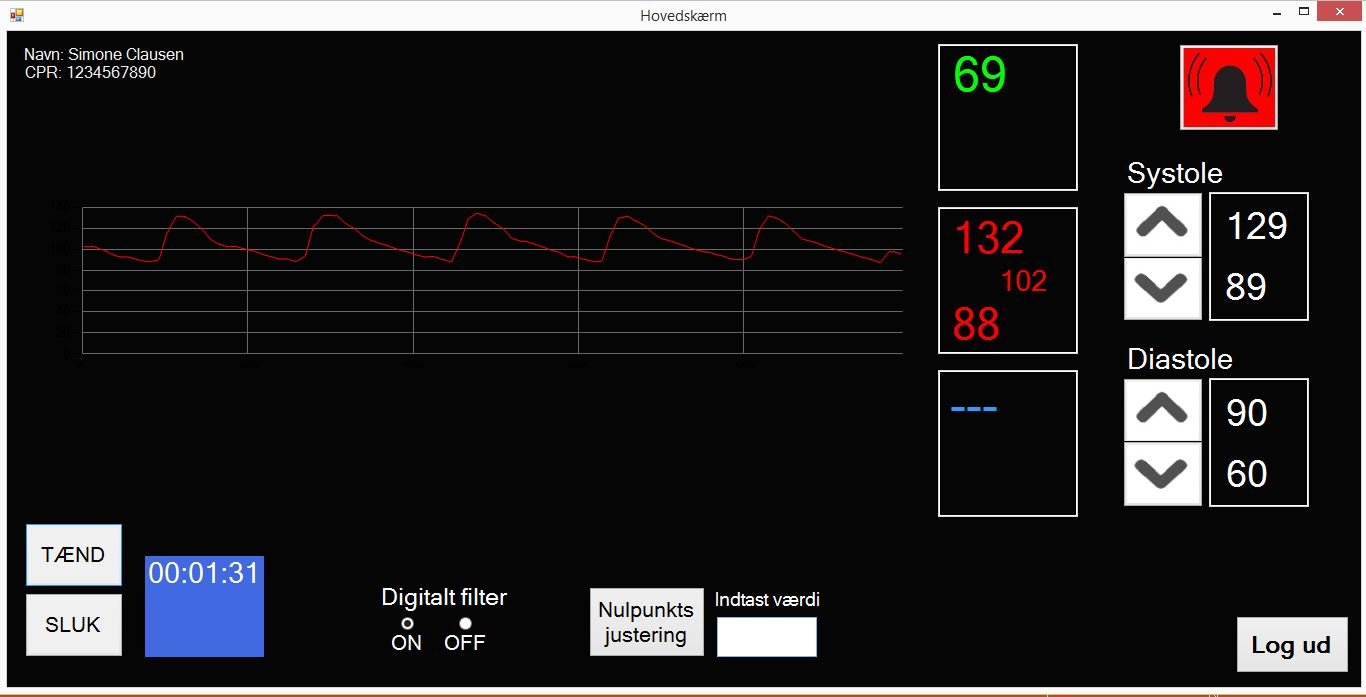
\includegraphics[width =0.6\textwidth , center]{billeder/IThovedGUIAlarm}
\caption{\textbf{Grænseværdi for systole ændret og alarm igangsat.}}
\end{figure}
I acceptesten for Use case 4, skal der trykkes på sluk, derefter log ud og til sidst ja på pop-up vinduet. På figuren nedenfor, ses det, at der er trykket på sluk-knappen, da den er blevet gennemsigtig, og det kun er tænd-knappen der kan trykkes. Log ud er blevet trykket på; "bekræft" pop-up vinduet kommer frem. Herved virker log ud knappen som den skal, og der bliver gemt målinger for patienten i EPJ-databasen. Blodtryksmålingen for patienten bliver gemt løbende i EPJ-databasen. 
\begin{figure}[H]
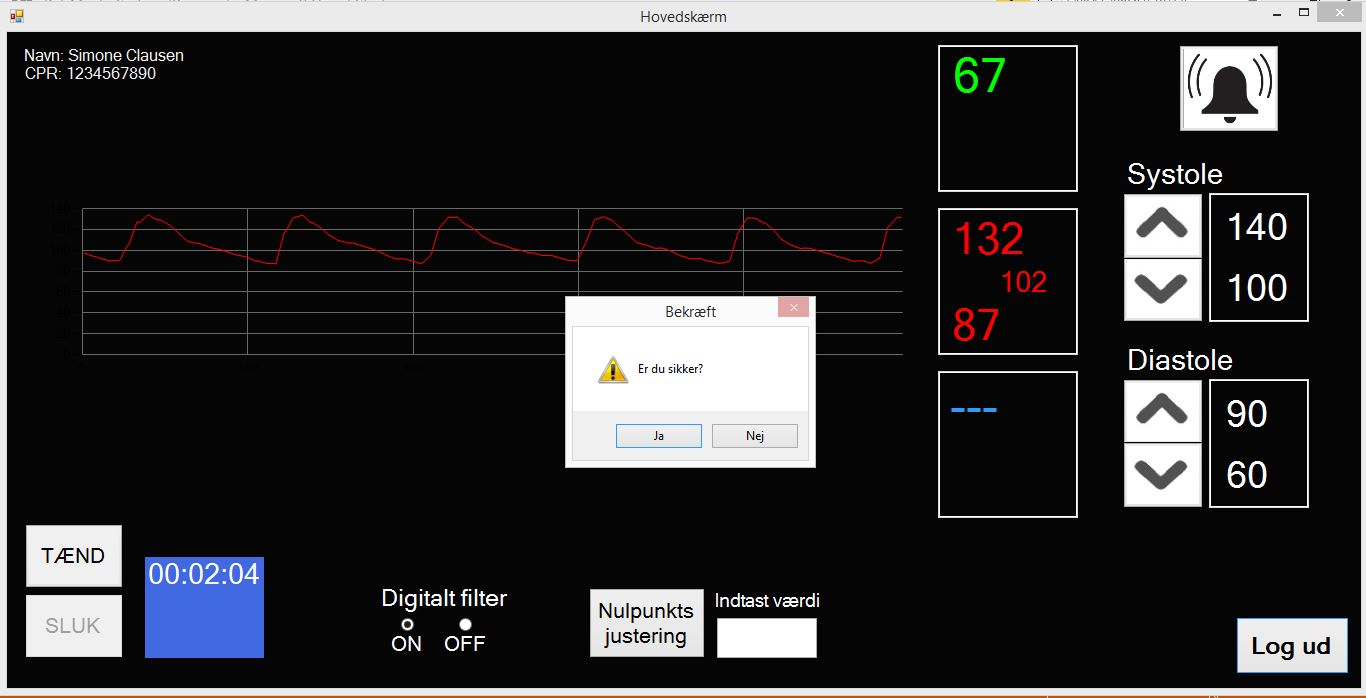
\includegraphics[width =0.6\textwidth , center]{billeder/IThovedGUILogUd}
\caption{\textbf{Log ud af blodtryksmålesystemet.}}
\end{figure}
Fra de foregående figur kan det konkluderes, at blodtryksmålesystemet lever op til accepttestens krav omkring, at kunne vise et blodtrykssignal kontinuert, samt slå et digitalt filter til og fra. \\\\
Blodtryksmålesystemet lever også op til kravet omkring at kunne kalibrere systemet. Dette gøres på startskærmen. Kravet til at systemet kan nulpunktsjusteres er ligeledes opfyldt, denne sker på hovedskærmen. Det kan diskuteres om det var smartere at systemet selv kan foretage nulpunktsjusteringen, end at man selv skal aflæse værdien. Nulpunktsjusterings knappen lever op til kravet om at kunne nulpunktsjustere blodtryksmålesystemet. \\\\
Grænseværdierne for blodtryksmålesystemet kan også ændres, herved er dette krav opfyldt, og der kommer en alarm når værdierne for enten systolen eller diastolen overskrider grænseværdierne. \\
Alarmen kan også udsættes i et minut, hvilket gøres ved at trykke på udsæt alarm knappen oppe i højre hjørne af hovedskærmen. 
\\\\
En anden ting som blodtryksmålesystemet også kan, er at vise en timer, som starter når man har trykket på start knappen. Denne timer stopper når der trykkes på sluk knappen. Det kan diskuteres, om timeren skal nulstilles, når der trykkes på start knappen igen. Det er valgt i dette projekt, at timeren fortsætter fra det stoppede tidspunkt, når tænd knappen bliver trykket igen. Dette er valgt, da man skal kunne fortsætte blodtryksmålingen.
\\\\
Det kan diskuteres om brugeren skal have lov til at kalibrere på startskærmen, da kalibreringen skal foretages af en servicemedarbejder. Herved skulle der kun have været log ind på startskærmen, og være lavet et servicevindue, som kun kan betjenes af servicemedarbejderen. Der er taget højde for denne problemstilling i koden, ved at have lavet en config fil, hvor kalibreringstallet kan ændres. Det betyder, at hvis det sundhedsfaglige personale springer over kalibreringen på startskærmen, kalibrerer systemet automatisk efter kalibreringstallet i config filen. Meningen med config filen er, at det kun er servicepersonalet, der skal kunne tilgå denne fil, og kunne ændre kalibreringstallet. 
\section{Udviklingsværktøjer}
Til udviklingen af produktet, og dermed igennem hele projektarbejdet, er der blevet brugt en række udviklingsværktøjer. I dette afsnit er disse udviklingsværktøjer beskrevet yderligere.
\subsection{Microsoft Visio 2010}
Tegneværktøjet Microsoft Visio, er blevet anvendt i forbindelse med design af både UML og SysML diagrammer. Microsoft Visio er det oplagte valg til at designe disse diagrammer, da programmet søger for at diagrammerne får et enkelt udseende og tydeligt kommunikerer til læseren, hvad diagrammerne vil vise.
\subsection{Visual Studio 2013}
Visual Studio 2013 er et udviklingsværktøj, designet til Microsoft .NET-frameworket. Dette udviklingsværktøj er specielt velegnet til design af brugergrænseflader, som i dette projekt er specifikt brugbart, da der skal udarbejdes et Windows Forms program.
\subsection{NI Multisim 13.0 med Ultiboard 13.0}
Til at designe hardwaren er Multisim med Ultiboard blevet benyttet. Multisim er et program der kan bruges ved kredsløbsdesign, da komponenterne her er lette at sætte i forhold til hinanden, da programmet indeholder samtlige komponenter, der skal benyttes i projektet. Ultiboard bruges til at designe printet, der skal bruges til at realisere hardwaren, der er blevet designet i Multisim. Ved at benytte Ultiboard undgås det at benytte et fumlebræt eller veroboard, hvor komponenterne skal kobles sammen med ledninger. Ved et print der designes med Ultiboard vil forbindelserne mellem komponenterne være direkte implementeret på printet og komponenterne vil derfor være nemme at implementere på printet.
\subsection{NI-DAQmx}
NI-DAQmx, også omtalt NI-DAQ/DAQ, er et værktøj som er blevet udarbejdet af National Instrument. Dette værktøj anvendes til at indsamle det indkommende signal. Dette signal kommer fra hardwaren. NI-DAQ omdanner desuden signalet fra et analogt signal til et digitalt signal, der kan bruges i koden. 
\subsection{Analog Discovery fra Digilent and Analog Devices}
Analog Discovery benyttes i projektet som en waveform-generator. Det er derfor Analog Discovery, der benyttes til at teste systemet. Dette sker ved at der sendes et blodtrykssignal fra Physionet.org ind i systemet, som systemet derefter skal behandle. Desuden er oscilloskopfunktionen i waveforms blevet benyttet under test af hardware.
\section{Opnåede erfaringer}
På baggrund af vores sundhedsfaglige viden og de opsatte rammer for projektet, er der blevet opstillet en projektformulering, som er løst ved hjælp af viden omkring programmering, analog og digital signalbehandling, SysML og UML. Arbejdet har styrket vores tværfaglige kompetencer og vi har formået at skabe en teknisk løsning på et sundhedsfagligt problem.\\
Kompetencerne indenfor digital signalbehandling, er indenfor dette projekt opnået ved at udarbejde et moving average lavpasfilter. Inden det blev klart at dette lavpasfilter skulle benyttes, er flere forskellige filtre blevet afprøvet. Disse filtre er ved brug af programmet MatLab blevet afprøvet, et butterworth IIR (Infinite impulse filter) lavpas filter her blev udarbejdet. Det var dog et FIR (Finite impulse filter) lavpasfilter der skulle benyttes, hvilket førte frem til at moving average filteret blev afprøvet, hvilket virkede efter hensigten. \\
Programmeringskoden til filteret skulle herefter udarbejdes, her blev der undersøgt forskellige metoder, der kunne benyttes via søgninger på internettet, hvilket sammen med pseudokode førte frem til at koden kunne skrives til det digitale filter. Realiseringen af lavpasfilteret forbedrede derfor ligeledes programmeringskompetencerne. Pseudokode blev brugt ved alle problemstillingerne i programmeringen, for at finde frem til den tilgang, der skulle bruges for at løse problemet. Bl.a. ved udarbejdelse af metoden til hvordan der skulle holdes styr på den data, der skulle sendes op, blev pseudokode benyttet. Idet blodtrykket skulle vises løbende, skulle der være en kømetode, som kunne indhente og udsende data løbende og samtidig holde styr på data i køen.\\
Andre softwarekompetencer er ligeledes blevet opnået, ved at benytte forskellige mønstre og kodeopbygninger, hvor netop kombinationen af disse faktorer har ført til en bredere forståelse i programmering og hvordan et projekt logisk kan bygges godt op. Herunder hvordan de forskellige metoder må ligge og hvordan klasserne må snakke sammen. \\\\
Data, der skulle sendes ind i koden, skulle først igennem den udarbejdede hardware. Under udarbejdelsen af hardware produktet er kompetencerne inden for analog signalbehandling, blevet forbedret. Ud fra problemstillingen og projektformuleringen vidste vi, hvordan signalet skulle sendes ind, her skulle kredsløbet, der skulle praktisere dette, først designes. En forstærker og et lavpasfilter skulle designes, hvilket blev gjort i forskellige faser. Igennem beregninger kunne komponenterne, der skulle benyttes ved forstærkeren og lavpasfilteret, bestemmes. Herefter kunne kredsløbet designes i multisim og på fumlebræt for at se om det analyserede kredsløbet kunne realiseres. \\\\
Det var lærerigt at give reviews til andre grupper, da vi her fik muligheden for at reflektere over, hvordan vi selv havde arbejdet med projektet og samtidig fik vi et indblik i, hvordan de andre grupper havde valgt at gribe opgaven an. Der blev udført to reviews, et review på kravspecifikation og accepttest, og et review på design og specifikation af software og hardware. \\ Desværre har der gennem projektforløbet været en del forvirring på tværs af grupperne omkring diverse krav og fremgangsmåder vedrørende projektudførelsen, hvilket gjorde review møderne mindre udbytterige end de kunne have været.\\\\
Projektstyringen og ledelsen må vi indse har været for svag i dette projekt. Oprindeligt ville vi have benyttet SCRUM, men dette kom ikke op at køre, så opgaverne har været mere løst defineret. Hvor vi igennem SCRUM kunne have identificeret mere klare opgaver og sat en fast deadline for, hvornår opgaven skulle være færdig. Ligeledes kunne opgaverne her prioriteres sådan det også blev identificeret hvor stor opgaven var og hvor høj prioritering denne opgave skulle have. Det må dog også erkendes at fordelingen af ressourcerne ikke har været optimalt. 
\section{Fremtidigt arbejde}
I dette projekt har der været flere overvejelser om, hvorledes vi ønskede vores slutprodukt skulle se ud og hvilke funktioner vi efterstræbte at opfylde. Vores besøg på Herning sygehus gav os et indblik i, hvordan en invasiv blodtryksmåler fungerer i praksis og hvilke funktioner, der er indbygget heri. Vi ønskede altså at basere vores system ud fra et virkeligt brugsscenarie. Dette brugte vi som udgangspunkt for vores system og vi udtænkte derfor en ide og opstillede et design, som vi ville udarbejde i vores projekt. Vores produkt skulle slutteligt kunne vise både EKG, blodtryk og iltmætning. Alle værdier skulle udskrives i en graf og talværdierne vises på brugergrænsefladen. 
\subsection{EKG-signal}
EKG-signalet skulle simuleres ved at sende et EKG-signal fra physionet.org via Analog Discovery ind i en anden port i DAQ’en. Dette signal skulle på lige fod med blodtryks-data præsenteres visuelt. Ligeledes skulle der være mulighed for at disse data kunne gemmes i databasen.
\subsection{Iltmætning}
Iltmætning ønskede vi at implementere i vores system, så dette, ligeledes som blodtrykket og EKG, ville blive præsenteret visuelt. For at få vist iltmætning, ville vi benytte et pulsoxymeter. Pulsoxymeteret sættes på fingeren og virker ved at gennemlyse fingeren med infrarødt lys. Herved måles iltmætningen i blodet. Disse data kunne via USB overføres til programmet. 
\subsection{EPJ}
Fremtidigt ville vi implementere vores system op mod eksisterende EPJ systemer, da vores system allerede er baseret på et virkeligt brugsscenarie, forventer vi, at en implementering ville være relativt enkel. Vores patientdata ville i stedet for vores database være hentet fra EPJ. Ligeledes vil vores logindata for sundhedsfaglig personale være hentet enten i Active Directory (netværket) eller i personaledatabasen. Blodtryksdata skulle stadig gemmes separat, men som vi kommer ind på i næste afsnit omkring datawarehouse, så skal data være kvalificeret af en række metadata.
\subsection{Datawarehouse}
Det blev fra projektets start talt om at lave et datawarehouse, realiseret med et slags mock-up datawarehouse til analysering af blodtryksmålinger. Et datawarehouse er en samling af data fra forskellige kilder, der er sorteret efter emne, i vores tilfælde ville det eksempelvis være blodtryksmåledata. Dette emne ville så være kvalificeret af en række dimensioner, repræsenteret af metadata i vores database.\\ 
Metadata / dimensioner kunne være ting som:
\begin{itemize}
\item Aldersgruppe eller alder
\item Køn
\item Datotid
\item SKS-koder (Sundhedsvæsnets Klassifikations System)
\item Behandlingssteder/Afdelinger
\item Andre metadata fra EPJ
\end{itemize}
Et datawarehouse fungerer absolut bedst, når der er akkumuleret mange data, da det giver et mere retvisende billede af tendenser. 
\chapter{Konklusion}
Vi kan i dette projekt konkludere, at der er blevet udarbejdet et system, som kan tilsluttes et væskefyldt kateter og vise en blodtrykskurve på en computerskærm. Igennem dette projekt ønskede vi, at opstille et system, som afspejler et hverdagsscenarie og efterlever de funktionaliteter, som vi fik fortalt og beskrevet af en anæstesisygeplejerske fra Herning Sygehus. Overordnet set, ønskede vi altså at opstille to systemer tilsvarende dem, som benyttes på sygehuse i dag. Et som skulle simulere EPJ systemet og et som skulle simulere den monitor, som bruges til afbildning af blodtryk, EKG og iltmætning. \\
\\
I vores system har vi implementeret de to systemer, som to skærme. Den første skærm, som vises i vores program er startskærmen, det er her personalet logger ind og vælger patienten. Derudover er det også her vi kalibrerer. Denne funktion skal udføres af en servicemedarbejder og ville i et hverdagsscenarie ikke ske i EPJ systemet. Når der er logget ind kommer vi til hovedskærmen. Her vises patientens navn og CPR, og det sundhedsfaglige personale kan starte blodtryksmålingen. I vores system var det tidsmæssigt og ressourcemæssig ikke mulig, at få implementeret EKG og iltmætning, og vi viser derfor kun blodtrykket, med systolisk, diastolisk og middeltryks værdier. På denne skærm har vi valgt, at nulpunktjustering skal kunne foretages, men er bevidste om, at dette ville ske automatisk og altså ikke er vist på en blodtryksmåler i praksis.  Vi har endvidere udarbejdet to databaser, en EPJ database og en personale database, som afspejler det EPJ system, der bruges i sundhedssektoren i dag. \\
\\
Vi kan efter denne projektproces konkludere, at vi har opnået det overordnede resultat og mål, som vi havde for vores system. Vi har igennem interaktion mellem hardware og software fået vist et blodtrykssignal, og der udskives systolisk og diastolisk tryk, som er indenfor de grænseværdier, der ses ved et normalt blodtryk. \\
\\
I forbindelse med procesledelse og -deltagelse, har vi i gruppen lært vigtigheden i at have en leder, som kan holde et overordnet overblik og tage styring og lederskab når dette er nødvendigt. Vi har i gruppen været seks mand, og det er derfor vigtig, at en fra holdet kan samle trådene og sørge for et fællesskab i gruppen, hvor alle yder samme indsats for samarbejdet og projektet. Vi har derfor også været nødsaget til samle gruppen og udnævne en ny leder, som turde tage de valg og det ansvar, som følger med lederrollen. Samlet set har vi i dette projekt opnået ny viden og draget værdifulde erfaringer, som vi kan tage med i et videre projekt arbejde. 
